% ============================================================
% ConsistXApp
% Revised manuscript
% Target journal: Annals of Telecommunications (sn-jnl.cls)
% ============================================================

\documentclass[pdflatex,sn-mathphys-num,iicol,oneside]{sn-jnl}

% ============================================================
% Packages
% ============================================================

\usepackage{amsmath}
\usepackage{amssymb}
\usepackage{bm}
\usepackage{booktabs}
\usepackage{array}
\usepackage{tikz}
\usepackage{url}
\usepackage{xurl}
\usepackage{graphicx}
\usepackage{float}
\usepackage{microtype}
\usepackage{xspace}
\usepackage{enumitem}

\usetikzlibrary{
  arrows.meta,
  positioning,
  fit,
  calc,
  shapes.geometric
}

% ============================================================
% Algorithms
% ============================================================

\floatstyle{ruled}
\newfloat{algorithm}{t}{loa}
\floatname{algorithm}{Algorithm}

\newcommand{\algin}[1]{\textbf{Input:} #1\par}
\newcommand{\algout}[1]{%
  \textbf{Output:} #1\par
  \vspace{2pt}\hrule\vspace{3pt}%
}

\newenvironment{algsteps}
  {\begin{enumerate}[
      leftmargin=1.8em,
      itemsep=1pt,
      parsep=0pt,
      topsep=2pt,
      label=\arabic*:
    ]}
  {\end{enumerate}}

% ============================================================
% Commands and theorem environments
% ============================================================

\newcommand{\method}{\textsc{ConsistXApp}\xspace}
\newcommand{\gac}{\textsc{GAC}\xspace}
\newcommand{\cpsat}{\textsc{CP-SAT}\xspace}

\newtheorem{proposition}{Proposition}
\newtheorem{definition}{Definition}
\newtheorem{remark}{Remark}

\raggedbottom

% ============================================================
% Document
% ============================================================

\begin{document}

\title[Verifier-Gated Multi-xApp Arbitration]{
Verifier-Gated and Auditable Multi-xApp Arbitration in the Near-RT RIC: Registered-Model Guarantees and the Limits of Incremental Repair
}

\author*[1]{\fnm{Lillia} \sur{Ouali}}
\email{lillia.ouali@univ-bejaia.dz}

\author[2]{\fnm{Madani} \sur{Bezoui}}
\email{mbezoui@cesi.fr}

\author[1]{\fnm{Kamal} \sur{Amroun}}
\email{kamal.amroun@univ-bejaia.dz}

\author[3]{\fnm{Ahcene} \sur{Bounceur}}
\email{abounceur@sharjah.ac.ae}

\affil*[1]{\orgdiv{Department of Computer Science}, \orgname{University of Bejaia}, \orgaddress{\city{Bejaia}, \country{Algeria}}}

\affil[2]{\orgdiv{LINEACT}, \orgname{CESI}, \orgaddress{\city{Nancy}, \country{France}}}

\affil[3]{\orgname{University of Sharjah}, \orgaddress{\city{Sharjah}, \country{United Arab Emirates}}}

% ============================================================
% Abstract
% ============================================================

\abstract{
Independently developed xApps may issue concurrent control requests
that are mutually incompatible or violate registered service-level
constraints. We formulate multi-xApp arbitration in the Near-RT RIC
as a dynamic finite-domain constraint problem and present \method, a
verifier-gated pipeline that binds each decision to a registered
model version and emits a replayable audit certificate (providing logical replayability without tamper-evidence unless cryptographic hashes are added) for every
repair. Upstream, incremental generalized arc consistency removes
unsupported values, while invalid candidates are repaired by solving
expanding local subproblems guided by propagation explanations,
solver infeasibility cores, or a deterministic graph frontier.
Across four validation gates comprising 680{,}450 checks, the
production verifier exhibited zero observed divergence from
independently implemented references. On 250 generated static
instances representing five O-RAN conflict scenarios, every
verifier-accepted outcome satisfied all registered hard constraints.
The latency benefit was amortized rather than absolute: under 2\%
sequential relation updates, repair of the previous accepted decision
required median per-epoch latencies of 0.05--4.9~ms for 100--1{,}000
variables, compared with 2.8--25.6~ms for the evaluated Python
\cpsat rebuild-and-resolve baseline. The advantage narrowed near the
pooled p95, reversed at the descriptive pooled p99, and disappeared
on cold starts. Local repair also reduced objective quality relative
to complete optimization. All guarantees are conditional on the
correctness and completeness of the registered constraint model and
do not establish physical-RAN safety or hard real-time
schedulability.
}

\keywords{
O-RAN,
xApp conflict management,
dynamic constraint satisfaction,
generalized arc consistency,
explanation-based repair,
constraint programming,
Near-RT RIC
}

\maketitle

% ============================================================
\section{Introduction}
\label{sec:introduction}
% ============================================================

The Open Radio Access Network (O-RAN) architecture disaggregates the
radio access network and exposes its control through programmable
components. Its near-real-time RAN Intelligent Controller (Near-RT
RIC) hosts xApps, namely third-party applications that subscribe to
measurements and issue control requests through the E2 interface
within control loops ranging from tens of milliseconds to one second
\cite{polese2023oran}. Because xApps may be developed independently,
often by different vendors, they may request incompatible values of
the same parameter, steer distinct parameters toward jointly
incompatible operating points, or collectively violate a
service-level agreement (SLA). The O-RAN Alliance therefore assigns a
conflict-mitigation function to the Near-RT RIC
\cite{oran2024conflict}. The associated literature commonly
distinguishes direct, indirect, and implicit conflicts and proposes
mechanisms for their detection and resolution
\cite{adamczyk2023conflict,wadud2024qacm}.

Most existing mechanisms primarily address what a candidate action
may do to the network through profiling, digital twins, learning, or
bargaining. This paper addresses the complementary
\emph{post-registration arbitration problem}: given finite action
domains and registered hard relations, construct and audit a joint
action such that no assignment violating the current registered model
version is admitted to the E2 control path.

Throughout, \emph{verified} means \emph{accepted by the registered-model
verifier}. It does not mean formally verified software: the paper
provides architectural, differential, exhaustive, property-based, and
mutation-based evidence for verifier correctness, not a machine-checked
proof of the verifier implementation.

The following vocabulary is used consistently. A \emph{proposal} is an
individual xApp request. A \emph{candidate} is a joint assignment
before verification. An \emph{accepted decision} is a candidate
accepted by the verifier. A \emph{forwarded action} is an accepted
decision actually admitted to the E2 control path. A
\emph{certificate} is the replayable audit object associated with a
repair.

We answer with \method, a coordination pipeline that combines three
established constraint-programming mechanisms in an O-RAN control
architecture. First, an incremental generalized arc-consistency
(\gac) stage removes values having no support in an incident hard
relation, reuses propagation state across decision epochs, and
restores affected values when a relation is relaxed. Second, when a
decoded candidate violates one or more relations, a solver-based
repair stage solves an induced subproblem. The violated constraints
seed a variable core, variables outside the core are fixed to the
candidate values, and the core expands according to propagation
explanations, solver infeasibility cores, or a deterministic frontier.
The repair may escalate to the complete model. Third, an independently
implemented verifier gates every forwarded action. The architecture is
deliberately conservative: optimizer output is treated as a proposal
until it has been checked against the current registered model.

The central contribution is a verifier-gated arbitration architecture
with model-version binding and replayable audit certificates (providing logical replayability without tamper-evidence);
incremental \gac and expanding local repair are upstream mechanisms
for generating acceptable candidates efficiently. The paper does not
claim a new consistency algorithm.

A complete modern constraint solver provides a strong baseline for
the generated instances considered here.
On the small static instances used in our scenario suite, rebuilding
and solving the complete \cpsat model requires less than 3~ms in the
median. Consequently, the approximately 1~ms median difference in
favour of \method on this suite is not, by itself, a compelling reason
to deploy an additional coordination layer. The intended operating
regime is sequential: consecutive decision epochs are expected to
share most of their variables, domains, and relations.

In the evaluated implementation, rebuilding a \cpsat model at every
epoch incurs model-construction and full-model search costs that scale
with the complete generated instance, and supplying the previous
solution as a hint did not materially reduce these costs. Repairing
the previous accepted decision instead operated on the relations
invalidated by the update and on the repair core induced by them. The
scope of this comparison---an evaluated Python rebuild-and-resolve
baseline, not every persistent or incremental solver architecture---is
detailed in Section~\ref{sec:baseline-scope}.

The contributions of this paper are as follows.

First, we implement and validate an independent forwarding verifier
for registered multi-xApp arbitration. The verifier is evaluated
through exhaustive comparison with an oracle, a second
implementation, property-based testing, and oracle-labelled input
mutation, with model-version binding tying every decision to the
registered model against which it was checked
(Section~\ref{sec:limitations} discusses the scope of this
evidence).

Second, we make every non-trivial arbitration auditable: each repair
emits a replayable certificate recording the violation witnesses, the
core-expansion trace and its causes, and the final verifier outcome.

Third, we formulate registered arbitration as a dynamic finite-domain
constraint problem with context-dependent hard relations, soft
utility, and temporal-stability costs, and we integrate established
constraint-programming mechanisms---incremental \gac with restoration,
explanation-guided monotone core expansion with conditional
completeness, and solver-based repair---into the verified pipeline.
Expanding cores resolved all 248 evaluated repair candidates, whereas
fixed violated-scope repair failed on 21 of them; this success-rate
difference is statistically significant under the exact paired test.
We also evaluate stronger conflict-aware decoders and show that they
reduce, but do not eliminate, the need for verified repair.

Finally, we characterize the operating regime and its limitations:
sequential repair provides a growing median advantage when updates
are small; there is no cold-start advantage over complete \cpsat up
to 1{,}000 variables; the available sample supports only descriptive
tail conclusions; local repair has a measurable objective-quality
cost; and an evaluated continuous-relaxation stage is
counterproductive.

Each contribution maps to a specific result, as summarized below.

\begin{enumerate}[label=(C\arabic*),leftmargin=2.4em]
\item \textbf{Verifier-gated architecture:}
Proposition~\ref{prop:soundness} and validation gates G1--G4
(Section~\ref{sec:verifier-gates}, Table~\ref{tab:gates}).
\item \textbf{Replayable audit certificate:} the certificate schema
and validity conditions of Definition~\ref{def:certificate}, with the
worked replay of Section~\ref{sec:certificate-example}.
\item \textbf{Expanding repair:} 248/248 candidates repaired by
expanding cores against 227/248 under fixed violated-scope repair
(Section~\ref{sec:repair-ablation}).
\item \textbf{Sequential operating regime:} median per-epoch
latencies and their tail limitations
(Section~\ref{sec:sequential}).
\item \textbf{Negative boundaries:} absence of a cold-start
advantage, the objective-quality gap, and the counterproductive
continuous relaxation (Sections~\ref{sec:sequential}
and~\ref{sec:objective-quality}).
\end{enumerate}

These contributions answer six research questions stated in
Section~\ref{sec:experiments}, each of which is addressed by a
corresponding results subsection.

Section~\ref{sec:background} reviews related work.
Section~\ref{sec:model} defines the coordination model.
Section~\ref{sec:method} presents \method, and
Section~\ref{sec:analysis} gives its formal properties.
Sections~\ref{sec:experiments} and~\ref{sec:results} describe the
experimental setup and results.
Section~\ref{sec:limitations} discusses threats to validity, and
Section~\ref{sec:conclusion} concludes the paper.

% ============================================================
\section{Background and Related Work}
\label{sec:background}
% ============================================================

The Near-RT RIC supports control loops between tens of milliseconds
and one second. xApps subscribe to key performance measurements
(KPMs), process network context, and issue E2 control requests
\cite{polese2023oran}. Experimental platforms such as ColO-RAN,
OpenRAN Gym, and FlexRIC support development and closed-loop
evaluation of O-RAN controllers
\cite{polese2022coloran,bonati2023openrangym,schmidt2021flexric}.

Three conflict classes are commonly distinguished
\cite{adamczyk2023conflict}. A \emph{direct conflict} occurs when two
xApps request incompatible values of the same controlled parameter.
An \emph{indirect conflict} occurs when different controlled
parameters influence a shared KPM. An \emph{implicit conflict}
couples distinct parameters and KPMs through network dynamics. Direct
conflicts can often be checked syntactically. Indirect and implicit
conflicts require a registered parameter--KPM dependency model, a
validated profile, a simulator, or a conservative operator rule.

Existing proposals include a conflict-mitigation framework integrated
into the RIC \cite{adamczyk2023conflict}, QoS-aware optimization that
maximizes the number of satisfied xApp requirements
\cite{wadud2024qacm,annals2024}, cooperative bargaining
\cite{wadud2023game}, pre-deployment profiling with statistical models
and hierarchical graphs \cite{prever2025pacifista},
digital-twin-based impact evaluation \cite{giannopoulos2025comix}, and
rule-based mitigation for mobility--energy interactions
\cite{wadud2025mobility}. XAI4C applies explainable-AI techniques to
conflict detection and mitigation \cite{varshney2025xai4c}. Its
explanations are post-hoc attributions of a learned mechanism,
whereas the explanations considered here are logical premises
replayable against a registered finite-domain model.

Table~\ref{tab:relatedwork} positions \method against the closest
representative systems along the dimensions that matter for
post-registration arbitration. The distinguishing combination is not
any single column but the conjunction of a hard-feasibility gate,
incremental repair, an audit trace, and model-version binding.

\begin{table*}[t]
\centering
\caption{Positioning of \method against representative conflict-management
systems. Entries reflect the mechanisms emphasized in the cited
descriptions; ``Not reported (n/r)'' denotes a property not reported as a design
element of that work rather than a demonstrated absence.}
\label{tab:relatedwork}
\setlength{\tabcolsep}{3.5pt}
\footnotesize
\begin{tabular}{
  >{\raggedright\arraybackslash}p{16mm}
  >{\raggedright\arraybackslash}p{30mm}
  >{\raggedright\arraybackslash}p{29mm}
  ccc c}
\toprule
Work &
Conflict classes &
Model basis &
\shortstack{Hard-\\feas.\\gate} &
\shortstack{Incr.\\repair} &
\shortstack{Audit\\trace} &
\shortstack{Version\\binding}\\
\midrule

QACM \cite{wadud2024qacm} &
Direct and indirect &
QoS-aware request optimization &
Not reported (n/r) & Not reported (n/r) & Not reported (n/r) & Not reported (n/r)\\

Bargaining \cite{wadud2023game} &
Direct and indirect &
Cooperative game-theoretic &
Not reported (n/r) & Not reported (n/r) & Not reported (n/r) & Not reported (n/r)\\

PACIFISTA \cite{prever2025pacifista} &
Direct, indirect, implicit &
Pre-deployment statistical profiling &
Not reported (n/r) & Not reported (n/r) & Profiles & Not reported (n/r)\\

COMIX \cite{giannopoulos2025comix} &
Indirect and implicit &
Digital-twin impact evaluation &
Not reported (n/r) & Not reported (n/r) & Not reported (n/r) & Not reported (n/r)\\

XAI4C \cite{varshney2025xai4c} &
Direct and indirect &
Learned model with post-hoc XAI &
Not reported (n/r) & Not reported (n/r) & Attributions & Not reported (n/r)\\

\midrule
\method &
Direct, indirect, implicit when registered &
Registered finite-domain model &
Yes & Yes & Yes & Yes\\

\bottomrule
\end{tabular}
\end{table*}

The comparison is deliberately narrow. These systems largely address
what a candidate action \emph{may do} to the network, a question
\method does not attempt to answer; conversely \method enforces a
registered model that those systems are, in part, mechanisms for
constructing. The approaches are therefore complementary rather than
competing, and the table should be read as a statement of scope, not
of superiority.

On the constraint-programming side, propagation removes domain values
that cannot participate in any locally supported tuple. For
non-binary relations, this property is generalized arc consistency,
which can be enforced efficiently for positive table constraints by
simple tabular reduction and related algorithms
\cite{yap2020gac,lecoutre2011str2}. Local consistency is not a
decision procedure: a \gac network may still be globally infeasible.
It can nevertheless detect some contradictions and reduce the search
space passed to a complete solver.

Dynamic constraint satisfaction studies sequences of related
problems and the incremental maintenance of consistency. A line of
work descending from DnAC-4 \cite{bessiere1991dynamic} maintains
per-value justifications so that, after a constraint retraction, only
a limited set of previously removed values must be reconsidered; AC$|$DC
\cite{berlandier1994acdc} and DnAC-6 \cite{debruyne1996dnac6} refine
this idea with lower space and time overheads. The restoration rule
used in this paper is deliberately coarser: after a relaxation, the
affected constraint-graph component is reset and re-filtered
(Section~\ref{sec:gac}). This choice trades restoration minimality
for simplicity of the audit trail, because component-level
restoration is directly replayable by the explanation checker without
per-value justification bookkeeping. We therefore position the
propagation layer as systems integration rather than as an
algorithmic advance over fine-grained dynamic arc-consistency
maintenance, which we neither extend nor benchmark against.
Explanation mechanisms record the causes
of value removals and contradictions and support diagnosis and
repair \cite{gupta2021explanations}. Dynamic backtracking
similarly preserves useful information while revising inconsistent
decisions \cite{ginsberg1993dynamic}. Large-neighbourhood search restricts a
complete solver to a neighbourhood of a current assignment and
modifies that neighbourhood as search proceeds
\cite{shaw1998lns}. Assumption-based infeasibility analysis identifies
a sufficient subset of active assumptions causing inconsistency; such
sets need not be cardinality-minimal.

Modern solvers such as OR-Tools \cpsat combine presolve, propagation,
clause learning, integer reasoning, and optimization
\cite{perron2023cpsat,ortools}. \method does not claim to invent
incremental consistency, explanations, assumption cores, or
neighbourhood repair. Its contribution is their integration with an
independently validated forwarding gate in registered xApp
arbitration, together with an evaluation that identifies the
sequential regime in which the integration was beneficial.

% ============================================================
\section{System Model}
\label{sec:model}
% ============================================================

\subsection{Epochs, actions, and registered relations}

The Near-RT RIC operates over decision epochs
$t=1,\ldots,T$. At epoch $t$, each active action variable
$i\in\mathcal{A}_t$ has a finite base domain
\begin{equation}
D_i^t=
\left\{
a_{i,1}^t,\ldots,a_{i,d_i}^t
\right\}.
\end{equation}
A value may encode acceptance or rejection of a request, a target
cell, an execution slot, a discrete power level, a handover offset, a
resource-allocation profile, or a registered no-operation. The
coordinated action is $x_i^t\in D_i^t$. The time index is omitted when
a single epoch is considered.

A constraint $c\in\mathcal{C}_t$ has a scope
$S_c\subseteq\mathcal{A}_t$ and an allowed relation
\begin{equation}
R_c(\bm{s}_t)
\subseteq
\prod_{i\in S_c}D_i^t,
\label{eq:relation}
\end{equation}
where $\bm{s}_t$ denotes the registered context. An assignment
$\bm{x}^t$ satisfies $c$ when
\begin{equation}
\bm{x}_{S_c}^t\in R_c(\bm{s}_t).
\end{equation}

Relations may be binary or higher-order and may be derived from
operator policies, ownership rules, SLA thresholds, validated xApp
profiles, simulators, digital twins, or conservative safety rules.
Hard constraints must be satisfied before forwarding. Soft
constraints contribute only to utility.

Let
$\mathcal{C}_{t,\mathrm{hard}}\subseteq\mathcal{C}_t$
denote the hard constraints. The registered hard model is
\begin{equation}
\mathcal{M}_t=
\left(
\mathcal{A}_t,
\bm{D}_t,
\mathcal{C}_{t,\mathrm{hard}},
\bm{s}_t,
\nu_t
\right),
\label{eq:model}
\end{equation}
where $\nu_t$ is a model-version identifier. A verification result is
valid only for the model version against which it was obtained. A
production implementation must therefore bind the decision,
certificate, and forwarding event to the same version and re-verify a
candidate if the registered model changes before forwarding.

Between epochs, xApps may activate or deactivate, domains and
constraints may change, relations may tighten or relax, and SLA
thresholds may move. The modified elements form a change set
$\Delta_t$. Restrictive and relaxing changes must be distinguished.
After a restriction, previous support information may remain useful.
After a relaxation, a previously removed value may have regained
support and must be reconsidered.

\subsection{Utility and temporal stability}

Let $u_i(a_i,\bm{s}_t)$ be the utility of choosing action $a_i$ for
variable $i$, with weight $\omega_i\geq 0$. Let $v_q\geq 0$ be a soft
violation with weight $\lambda_q\geq 0$. The static utility is
\begin{equation}
U(\bm{x},\bm{s}_t)
=
\sum_{i\in\mathcal{A}_t}
\omega_i u_i(x_i,\bm{s}_t)
-
\sum_{q\in\mathcal{Q}_t}
\lambda_q v_q(\bm{x},\bm{s}_t).
\label{eq:static-utility}
\end{equation}

Given the previous accepted decision $\bm{x}^{t-1}$ and
reconfiguration costs $\kappa_i\geq 0$, the weighted action churn is
\begin{equation}
H(\bm{x}^{t},\bm{x}^{t-1})
=
\sum_{i\in\mathcal{A}_t\cap\mathcal{A}_{t-1}}
\kappa_i
\mathbf{1}
\left[
x_i^t\neq x_i^{t-1}
\right].
\label{eq:churn}
\end{equation}

The general scalarized coordination problem is
\begin{align}
\max_{\bm{x}^{t}}\quad&
U(\bm{x}^{t},\bm{s}_t)
-
\mu H(\bm{x}^{t},\bm{x}^{t-1})
\label{eq:problem-objective}\\
\text{s.t.}\quad&
x_i^t\in D_i^t,
&& i\in\mathcal{A}_t,
\nonumber\\
&
\bm{x}_{S_c}^t\in R_c(\bm{s}_t),
&& c\in\mathcal{C}_{t,\mathrm{hard}},
\label{eq:problem-hard}
\end{align}
where $\mu\geq 0$ controls the preference for temporal stability. In this formulation, utility can compensate for additional churn depending on $\mu$.
However, the operational pipeline proposed in this paper implements a strictly lexicographic repair policy (Section~\ref{sec:repair}) where no utility improvement can compensate for any increase in primary churn. The complete-objective baseline evaluated in Section~\ref{sec:objective-quality} optimizes the lexicographic formulation
using the complete \cpsat model directly on the raw state. Dwell-time and cooldown rules are represented as hard relations when
their violation is not permitted.

\begin{table}[t]
\centering
\caption{Principal notation used throughout the paper.}
\label{tab:notation}
\footnotesize
\setlength{\tabcolsep}{3pt}
\begin{tabular}{@{}l>{\raggedright\arraybackslash}p{42mm}@{}}
\toprule
Symbol & Meaning\\
\midrule
$t$, $T$ & Decision epoch index and horizon\\
$\mathcal{A}_t$ & Active action variables at epoch $t$\\
$D_i^t$, $d_i$ & Finite base domain of variable $i$ and its size\\
$x_i^t$, $\bm{x}^t$ & Coordinated action value and joint assignment\\
$\mathcal{C}_t$, $\mathcal{C}_{t,\mathrm{hard}}$ & Constraints and hard constraints\\
$c$, $S_c$, $R_c(\bm{s}_t)$ & Constraint, its scope, its allowed relation\\
$\bm{s}_t$ & Registered context\\
$\mathcal{M}_t$, $\nu_t$ & Registered hard model and its version identifier\\
$\Delta_t$ & Change set between epochs $t-1$ and $t$\\
$u_i$, $\omega_i$ & Per-variable utility and its weight\\
$v_q$, $\lambda_q$, $\mathcal{Q}_t$ & Soft violation, weight, and soft-constraint set\\
$H$, $\kappa_i$, $\mu$ & Action churn, reconfiguration cost, stability weight\\
$U$ & Static utility of an assignment\\
$\mathcal{A}_r$ & Repair core (variables reoptimized during repair)\\
$\mathcal{X}_t$ & Verifier input representation space\\
$\mathcal{F}(\bm{s}_t)$ & Feasible set of the registered hard model\\
\bottomrule
\end{tabular}
\end{table}

\subsection{Worked example}
\label{sec:worked-example}

Consider a coverage xApp controlling

\[
x_1\in
\{
\text{low},
\text{medium},
\text{high}
\}
\]
and an energy-saving xApp controlling

\[
x_2\in
\{
\text{sleep},
\text{on}
\}.
\]
Suppose the registered relation is
\begin{equation}
R_{12}
=
\{
(\text{medium},\text{on}),
(\text{high},\text{on}),
(\text{low},\text{sleep})
\}.
\end{equation}

The relation forbids high power when the cell is sleeping and low
power when the cell is active. Assume that the preferred requests are
$x_1=\text{high}$ and $x_2=\text{sleep}$. These requests are soft
preferences; the base domains remain multivalued.

\gac removes no value. The value \text{high} has support
$(\text{high},\text{on})$, and \text{sleep} has support
$(\text{low},\text{sleep})$. Nevertheless, the independently decoded
pair
$(\text{high},\text{sleep})$ violates $R_{12}$. The verifier rejects
it, the violated relation seeds the repair core
$\{x_1,x_2\}$, and repair may return
$(\text{high},\text{on})$ or $(\text{low},\text{sleep})$ depending on
the registered preferences. Thus propagation removes individually
unsupported values, whereas repair resolves incompatible
combinations of individually supported values.

\subsubsection*{Certificate emitted by this repair}
\label{sec:certificate-example}

Assuming the registered preferences select $(\text{high},\text{on})$,
the arbitration above emits the following certificate:

\begin{verbatim}
model_version:      nu17
candidate:          (high, sleep)
violated_relation:  R12
initial_core:       {x1, x2}
expansion_trace:    none
final_assignment:   (high, on)
solver_status:      OPTIMAL
verifier_status:    ACCEPT
\end{verbatim}

Replaying this certificate under Definition~\ref{def:certificate}
requires checking that the recorded initial violation is reproducible
and that the final assignment is feasible, that is,
\begin{equation}
(\text{high},\text{sleep})\notin R_{12},
\qquad
(\text{high},\text{on})\in R_{12},
\end{equation}
both of which hold by inspection of $R_{12}$. The empty expansion
trace is consistent because the initial core already spanned every
variable of the violated relation, so no expansion was required. An
auditor can perform these checks without access to the solver, the
decoder, or the propagation engine.

% ============================================================
\section{The \method Framework}
\label{sec:method}
% ============================================================

Figure~\ref{fig:architecture} positions \method in the Near-RT RIC
control path. The pipeline separates four stages whose boundaries are
maintained throughout the paper:

\begin{enumerate}[label=\arabic*.,leftmargin=1.6em]
\item \textbf{Candidate generation:} incremental \gac followed by a
decoder, or, in the sequential regime, the previous accepted
decision.
\item \textbf{Repair feasibility:} expansion of a repair core solved
with objective-free \cpsat, establishing hard feasibility only.
\item \textbf{Operational optimization:} sequential lexicographic
optimization restricted to the retained core.
\item \textbf{Independent verification:} a full registered-model
membership test on the resulting candidate, followed by the
forwarding gate.
\end{enumerate}

Keeping these stages distinct avoids conflating four different
claims: finding a feasible core, optimizing within that core,
certifying optimality, and verifying hard feasibility. Only the
fourth stage supports the forwarding guarantee.

\begin{figure*}[t]
\centering
\resizebox{\textwidth}{!}{%
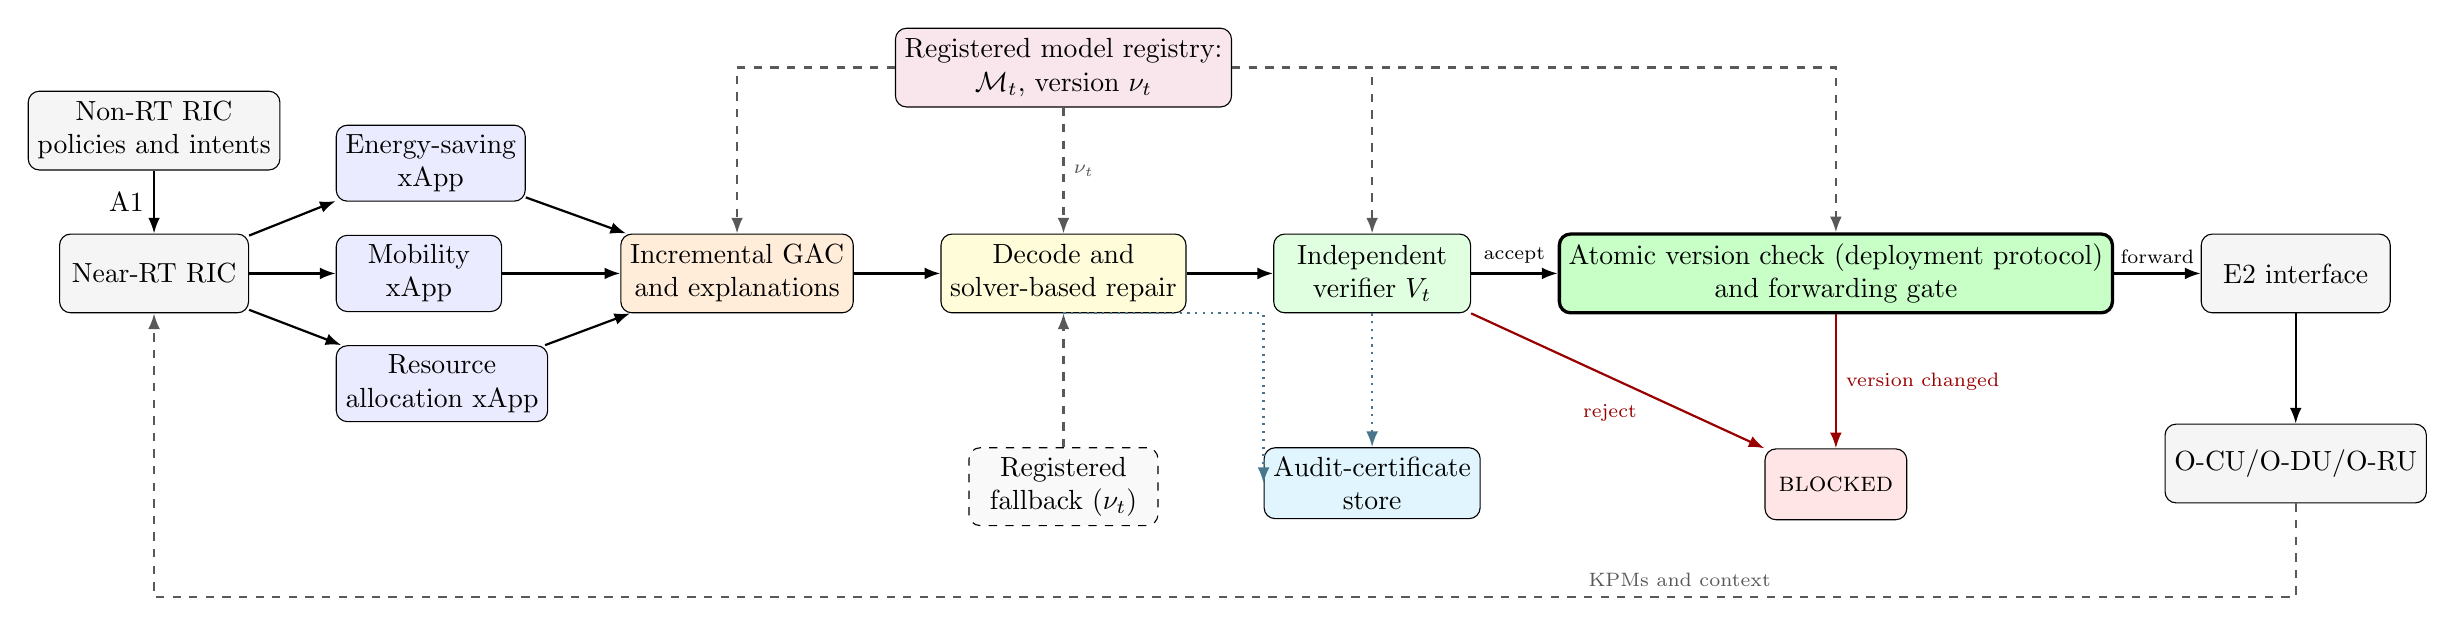
\begin{tikzpicture}[
  node distance=8mm and 11mm,
  block/.style={
    draw,
    rounded corners,
    align=center,
    minimum width=24mm,
    minimum height=10mm,
    fill=gray!8
  },
  app/.style={
    draw,
    rounded corners,
    align=center,
    minimum width=21mm,
    minimum height=9mm,
    fill=blue!8
  },
  prop/.style={
    draw,
    rounded corners,
    align=center,
    minimum width=26mm,
    minimum height=10mm,
    fill=orange!15
  },
  coord/.style={
    draw,
    rounded corners,
    align=center,
    minimum width=27mm,
    minimum height=10mm,
    fill=yellow!15
  },
  verify/.style={
    draw,
    rounded corners,
    align=center,
    minimum width=25mm,
    minimum height=10mm,
    fill=green!12
  },
  gate/.style={
    draw,
    very thick,
    rounded corners,
    align=center,
    minimum width=25mm,
    minimum height=10mm,
    fill=green!22
  },
  registry/.style={
    draw,
    rounded corners,
    align=center,
    minimum width=30mm,
    minimum height=10mm,
    fill=purple!10
  },
  store/.style={
    draw,
    rounded corners,
    align=center,
    minimum width=24mm,
    minimum height=9mm,
    fill=cyan!12
  },
  fallb/.style={
    draw,
    dashed,
    rounded corners,
    align=center,
    minimum width=24mm,
    minimum height=9mm,
    fill=gray!5
  },
  blocked/.style={
    draw,
    rounded corners,
    align=center,
    minimum width=18mm,
    minimum height=9mm,
    fill=red!10
  },
  arrow/.style={
    -{Latex[length=2mm]},
    thick
  },
  modelarrow/.style={
    -{Latex[length=2mm]},
    thick,
    dashed,
    gray!70!black
  },
  auditarrow/.style={
    -{Latex[length=2mm]},
    thick,
    dotted,
    cyan!50!black
  }
]

\node[block] (nonrt) {Non-RT RIC\\policies and intents};
\node[block,below=of nonrt] (near) {Near-RT RIC};

\node[app,right=of near,yshift=14mm] (x1)
  {Energy-saving\\xApp};
\node[app,right=of near] (x2)
  {Mobility\\xApp};
\node[app,right=of near,yshift=-14mm] (x3)
  {Resource\\allocation xApp};

\node[prop,right=15mm of x2] (gac)
  {Incremental GAC\\and explanations};

\node[coord,right=of gac] (coord)
  {Decode and\\solver-based repair};

\node[verify,right=of coord] (verifier)
  {Independent\\verifier $V_t$};

\node[gate,right=of verifier] (gate)
  {Atomic version check (deployment protocol)\\and forwarding gate};

\node[block,right=of gate] (e2)
  {E2 interface};

\node[block,below=14mm of e2] (ran)
  {O-CU/O-DU/O-RU};

% --- registry, certificate store, fallback, blocked ---
\node[registry,above=16mm of coord] (registry)
  {Registered model registry:\\$\mathcal{M}_t$, version $\nu_t$};

\node[store,below=17mm of verifier] (certstore)
  {Audit-certificate\\store};

\node[fallb,below=17mm of coord] (fallback)
  {Registered\\fallback ($\nu_t$)};

\node[blocked,below=17mm of gate] (blocked)
  {\textsc{blocked}};

% --- control proposal flow (solid) ---
\draw[arrow] (nonrt) -- node[left]{A1} (near);
\draw[arrow] (near) -- (x1);
\draw[arrow] (near) -- (x2);
\draw[arrow] (near) -- (x3);
\draw[arrow] (x1) -- (gac);
\draw[arrow] (x2) -- (gac);
\draw[arrow] (x3) -- (gac);
\draw[arrow] (gac) -- (coord);
\draw[arrow] (coord) -- (verifier);
\draw[arrow] (verifier) -- node[above,font=\scriptsize]{accept} (gate);
\draw[arrow] (gate) -- node[above,font=\scriptsize]{forward} (e2);
\draw[arrow] (e2) -- (ran);

% --- model/context data (dashed) ---
\draw[modelarrow] (registry.south) -- node[right,font=\scriptsize]{$\nu_t$} (coord.north);
\draw[modelarrow] (registry.west) -| (gac.north);
\draw[modelarrow] (registry.east) -| (verifier.north);
\draw[modelarrow] (registry.east) -| (gate.north);
\draw[modelarrow] (fallback.north) -- (coord.south);

% --- audit data (dotted) ---
\draw[auditarrow] (coord.south) -| (certstore.west);
\draw[auditarrow] (verifier.south) -- (certstore.north);

% --- rejection / blocked paths ---
\draw[arrow,red!60!black] (verifier.south east) --
  node[below left,font=\scriptsize,pos=0.6]{reject} (blocked.north west);
\draw[arrow,red!60!black] (gate.south) --
  node[right,font=\scriptsize]{version changed} (blocked.north);

% feedback routed below the whole diagram to avoid crossing the pipeline
\coordinate (fbLow) at ($(fallback.south)+(0,-9mm)$);
\draw[modelarrow]
  (ran.south) |- (fbLow)
  node[pos=0.75,above,font=\scriptsize]{KPMs and context}
  -| (near.south);

\end{tikzpicture}
}
\caption{
\method in the Near-RT RIC control path. Solid arrows carry control
proposals and accepted actions; dashed arrows carry registered-model
and context data; dotted arrows carry audit data. Every forwarded
action passes the independent verifier $V_t$ and an atomic
model-version check bound to $\nu_t$: a candidate rejected by the
verifier, or one whose model version changed between verification and
forwarding, is not admitted to E2. Incremental \gac and solver-based
repair generate candidates efficiently but are outside the trusted
path---a fault in either can reduce availability or objective
quality, but cannot by itself cause a registered-model-invalid
forwarding.
}
\label{fig:architecture}
\end{figure*}

\subsection{Incremental consistency filtering}
\label{sec:gac}

The propagator maintains a base domain $D_i$ and a filtered domain
$D_i^{*}\subseteq D_i$ for every variable. Keeping them separate is
necessary because a later relaxation may restore support for a value
that was previously removed.

For $a\in D_i$ and constraint $c$, the support set is
\begin{equation}
\begin{split}
\operatorname{Supp}_{c}
(i,a;\bm{D})
={}&
\bigl\{
\bm{z}\in R_c(\bm{s}_t):
z_i=a
\ \land\\
&\ \
z_j\in D_j,\
\forall j\in S_c
\bigr\}.
\end{split}
\label{eq:support}
\end{equation}

A hard network is generalized arc consistent when every value of
every variable has at least one support in every incident relation.
The revision operator is
\begin{equation}
\begin{split}
&\operatorname{Revise}_{c,i}(\bm{D}):
\\
&\quad
D_i
\leftarrow
\left\{
a\in D_i:
\operatorname{Supp}_{c}(i,a;\bm{D})
\neq\varnothing
\right\}.
\end{split}
\label{eq:revise}
\end{equation}

Revision is applied through a work queue until the fixed point
\begin{equation}
\bm{D}^{*}
=
\operatorname{GAC}
\left(
\bm{D},
\mathcal{C}_{\mathrm{hard}},
\bm{s}_t
\right)
\end{equation}
is reached. An empty filtered domain is a \emph{wipeout} and proves
that no feasible assignment extends the current domains. Non-empty
filtered domains do not prove global feasibility.

Across epochs, the propagator is incremental. The queue is seeded
with the constraints affected by $\Delta_t$ and constraints incident
to an affected variable. Under purely restrictive changes, cached
supports and previous deletions can be reused when their premises
remain valid. If the update contains a relaxation, the affected
constraint-graph component is restored to its base domains and
current allowed tuples before \gac is re-established. This
full-component restoration is a conservative sufficient rule; it is
not claimed to be the minimum restoration set computed by
fine-grained dynamic arc-consistency schemes
\cite{bessiere1991dynamic,berlandier1994acdc,debruyne1996dnac6}, and
is preferred here because the restored set is replayable by the
explanation checker without per-value justification state.

For explicit positive tables, the implementation records active
tuples, the last known support of each variable--value pair, the
context identifier under which the support was valid, and the
explanation attached to each removal.

\begin{algorithm}[t]
\caption{Incremental GAC with restoration after relaxation}
\label{alg:incgac}
\small

\algin{
warm filtered domains $\bm{D}^{*}_{t-1}$,
base domains, active tables, and change set $\Delta_t$
}

\algout{
filtered domains $\bm{D}^{*}_{t}$ or \textsc{wipeout}
}

\begin{algsteps}

\item Classify $\Delta_t$ as restrictive, relaxing, mixed, or
utility-only.

\item If $\Delta_t$ contains a relaxation, restore the affected
constraint-graph component to its base domains and current allowed
tuples.

\item Apply valid restrictive deletions to the warm domains.

\item Seed the work queue with changed constraints and constraints
incident to changed variables.

\item While the queue is non-empty, remove a constraint $c$ and revise
each $i\in S_c$.

\item If some revised domain becomes empty, return \textsc{wipeout}
with its explanation.

\item Whenever a domain shrinks, enqueue the constraints incident to
that domain.

\item Return the fixed-point domains $\bm{D}^{*}_{t}$.

\end{algsteps}
\end{algorithm}

\subsection{Propagation explanations}
\label{sec:explanations}

When a value $a$ is removed from $D_i$ by constraint $c$, the
propagator records an explanation
\begin{equation}
\mathcal{E}(i,a)
\subseteq
\mathcal{C}_{\mathrm{hard}}
\cup
\mathcal{L},
\end{equation}
where $\mathcal{L}$ contains temporary domain restrictions and
boundary decisions.

The explanation contains premises sufficient to establish that every
tuple of $R_c$ assigning $a$ to $x_i$ is inactive. For each candidate
support tuple, at least one recorded premise explains why the tuple
cannot be used. A wipeout explanation is
\begin{equation}
\mathcal{E}_{\emptyset}(i)
=
\bigcup_{a\in D_i}
\mathcal{E}(i,a).
\end{equation}

Explanations are not required to be cardinality-minimal. They must be
valid relative to the registered model, reproducible from the
propagation trace, associated with a model/context identifier, and
accepted by a separate explanation checker. The checker replays the
premises and verifies that every potential supporting tuple is
disabled.

\subsection{Decoding and explanation-guided solver-based repair}
\label{sec:repair}

If propagation terminates without a wipeout, a deterministic decoder
selects
\begin{equation}
\widehat{x}_i\in D_i^{*}
\end{equation}
as the highest-utility value under a documented tie-breaking rule.
This utility decoder is intentionally conflict-unaware and is used to
isolate the contribution of repair. Section~\ref{sec:decoder-baselines}
separately evaluates conflict-aware candidate generators.

Every decoded candidate is checked against all hard relations. Let
\begin{equation}
\mathcal{C}^{0}
=
\left\{
c:
\widehat{\bm{x}}_{S_c}
\notin
R_c(\bm{s}_t)
\right\}
\end{equation}
be the initially violated relations. The initial variable core is
\begin{equation}
\mathcal{A}^{0}
=
\bigcup_{c\in\mathcal{C}^{0}}S_c.
\end{equation}

At repair iteration $r$, variables outside
$\mathcal{A}^{r}$ are fixed to their decoded values, while variables
inside the core retain their filtered domains. \gac is enforced on
the restricted model before the subproblem is submitted to \cpsat.
A variable $j\notin\mathcal{A}^{r}$ that participates in a constraint
whose scope intersects $\mathcal{A}^{r}$ is called a
\emph{boundary variable} of iteration $r$.

Two further objects are used by the expansion rule. Let
$\operatorname{VarLit}(\mathcal{E})$ denote the set of variables
appearing in the temporary restriction literals or boundary decisions
contained in an explanation $\mathcal{E}$, and let
$\mathcal{E}_{\emptyset}^{r}$ denote the wipeout explanation recorded
at iteration $r$, that is, the set of literals whose conjunction
entails the empty domain. The set $\mathcal{C}^{r+1}$ denotes the
relations found violated or wiped out at iteration $r$ and used to
seed the next core.

The \emph{deterministic frontier rule} is defined as follows.
Constraints are indexed once, at model registration, by a fixed total
order (ascending registered constraint identifier). Adjacency is
taken through the constraint hypergraph, in which two variables are
adjacent when they co-occur in the scope of some active hard
relation. At each frontier expansion, the rule adds exactly one
constraint: the lowest-indexed active hard relation whose scope
intersects $\mathcal{A}^{r}$ but is not contained in it, together
with all variables in that scope. Ties cannot arise because the
constraint index is a total order. One constraint, not one adjacency
layer, is added per iteration; this keeps expansions minimal and
makes certificate replay deterministic.

If propagation produces a wipeout, its explanation supplies
constraints and variables for expansion:
\begin{equation}
\mathcal{A}^{r+1}
=
\mathcal{A}^{r}
\cup
\operatorname{VarLit}
\left(
\mathcal{E}_{\emptyset}^{r}
\right)
\cup
\bigcup_{c\in\mathcal{C}^{r+1}}S_c,
\label{eq:variable-expansion}
\end{equation}
where
\begin{equation}
\mathcal{C}^{r+1}
=
\mathcal{E}_{\emptyset}^{r}
\cap
\mathcal{C}_{\mathrm{hard}}.
\end{equation}

If propagation succeeds but the restricted model is reported
\texttt{INFEASIBLE}, the assumption-core variant uses reified
boundary fixings. For each boundary variable $j$, a Boolean assumption
literal $b_j$ enforces
\begin{equation}
b_j
\Rightarrow
\left(
x_j=\widehat{x}_j
\right).
\end{equation}

The literals returned by
\texttt{SufficientAssumptionsForInfeasibility} form a sufficient, not
necessarily minimum, set of assumptions whose simultaneous activation
is inconsistent with the remaining model. The corresponding boundary
variables are released. If the returned set is empty, all currently
fixed boundary variables are conservatively released. A solver status
of \texttt{UNKNOWN} is not interpreted as infeasibility.

The core-extraction model is a feasibility model and contains no
objective. In the default explanation-guided variant, boundary values
are represented by equality constraints. If neither an explanation
nor an assumption core adds a variable, a deterministic frontier rule
adds adjacent constraints and their variables.

\begin{algorithm}[H]
\caption{Explanation-guided repair-core expansion}
\label{alg:repair}
\small

\algin{
decoded candidate $\widehat{\bm{x}}$,
registered hard model,
stage-boundary experimental budget,
and the registered fallback associated with the current model version
}

\algout{
verified local repair,
verified full-scope repair,
verified registered fallback,
or \textsc{blocked}
}

\begin{algsteps}

\item \textbf{Core feasibility phase:} Compute the violated relation set $\mathcal{C}^{0}$ and set $\mathcal{A}^{0} \leftarrow \bigcup_{c\in\mathcal{C}^{0}}S_c$.

\item For repair iteration $r=0,1,\ldots$, fix each boundary variable $j\notin\mathcal{A}^{r}$ to $\widehat{x}_j$.

\item Enforce \gac on the restricted model.

\item If propagation wipes out at the full core $\mathcal{A}^{r}=\mathcal{A}_t$, the registered hard model is infeasible; no same-model candidate, including the registered fallback, can pass the verifier, so return \textsc{blocked} for the current model version.

\item If propagation wipes out on a proper core $\mathcal{A}^{r}\subsetneq\mathcal{A}_t$, extract the wipeout explanation, expand the core, and continue.

\item Otherwise solve the objective-free restricted subproblem with \cpsat.

\item If the solver reports \texttt{INFEASIBLE} at the full core $\mathcal{A}^{r}=\mathcal{A}_t$, the registered hard model is infeasible under the current exact encoding and conclusive status; return \textsc{blocked} for the current model version.

\item If the solver reports \texttt{INFEASIBLE} on a proper core, expand the core using an assumption core when available; otherwise use the deterministic frontier rule, and continue.

\item If the solver returns \texttt{UNKNOWN}, no infeasibility conclusion is drawn; invoke the registered fallback policy (since an UNKNOWN status typically indicates that the solver budget or deadline has expired) and go to the verification phase with the fallback candidate.

\item If the solver returns \texttt{FEASIBLE} or \texttt{OPTIMAL}, retain the current core $\mathcal{A}^{r}$ and break to the optimization phase.

\item \textbf{Operational optimization phase:} Optimize the lexicographic objectives on the feasible core. If every active lexicographic level returns \texttt{OPTIMAL}, mark the repair \textsc{lex-optimal}. If the remaining optimization budget expires after the solver has produced a feasible incumbent but before all lexicographic levels are certified, mark the result \textsc{feasible-not-certified} and submit the incumbent to the independent verification phase. The incumbent is not treated as verified at this point; independent verification occurs only in Step~12.

\item \textbf{Verification phase:} Submit the final optimized or fallback candidate to the independent verifier. If the verifier accepts it, return the verified candidate. If it rejects an optimized candidate, submit the registered fallback to the verifier; if the fallback is accepted, return it. Otherwise return \textsc{blocked}.

\end{algsteps}
\end{algorithm}

Each non-trivial arbitration emits a \emph{replayable audit
certificate} containing sufficient information to reconstruct the
initial violations, validate each recorded core expansion, and
recheck final registered-model feasibility. Concretely, the
certificate records the model and context identifiers, the decoded
candidate, the initial violation witnesses, the repair-core sequence,
the source of every expansion, the released boundary variables, the
final assignment, the solver status, and the verifier outcome.
Propagation explanations and solver assumption cores are included
when they cause an expansion. The certificate does not prove
minimum-core size, solver correctness, or global objective
optimality.

\begin{definition}[Certificate validity]
\label{def:certificate}
A certificate $\pi$ is \emph{valid} for the registered model
$\mathcal{M}_t$ at version $\nu_t$ when all of the following hold:
\begin{enumerate}[label=(\arabic*),leftmargin=2.0em]
\item the model and context identifiers recorded in $\pi$ match
$(\mathcal{M}_t,\nu_t)$;
\item the listed initial violations are reproducible by evaluating
the recorded candidate against the registered relations;
\item every recorded expansion follows the declared explanation,
assumption-core, or deterministic frontier rule;
\item all released boundary variables are recorded;
\item the final assignment is complete and domain-valid;
\item every registered hard relation is satisfied by the final
assignment;
\item the recorded verifier outcome and the forwarded assignment
agree.
\end{enumerate}
\end{definition}

Certificate validity establishes replayable registered-model
feasibility and trace consistency. It does not establish solver
optimality, physical-network safety, or completeness of the
registered model. The present evaluation did not separately measure
serialized certificate size or replay latency.

The intended repair preference order is lexicographic:

\begin{enumerate}
\item satisfy every hard relation;
\item minimize weighted reconfiguration against the previous verified
decision;
\item minimize deviation from the decoded candidate;
\item maximize static utility.
\end{enumerate}

Hard feasibility is not scalarized with the soft levels. A
\texttt{FEASIBLE} solver status establishes feasibility but does not
establish objective optimality. A claim of global objective
optimality requires a corresponding \texttt{OPTIMAL} status for the
encoded complete model. Accordingly, this paper uses
the term \emph{solver-based repair} for the \cpsat-based repair
engine. The evaluation therefore reserves \emph{certified optimum} (qualified by the exact encoded model, integer scaling of utilities, and active lexicographic levels)
for solutions proven optimal across all active lexicographic levels.
Table~\ref{tab:solver-status} states the conclusion permitted by each
solver status.

\begin{table}[t]
\centering
\caption{Permitted conclusions per solver status.}
\label{tab:solver-status}
\setlength{\tabcolsep}{4pt}
\small
\begin{tabular}{ll}
\toprule
Status & Permitted conclusion\\
\midrule
\texttt{OPTIMAL} &
\shortstack[l]{Feasible and optimal for the\\current encoded objective}\\[2pt]
\texttt{FEASIBLE} &
\shortstack[l]{Feasible incumbent; optimality\\not established}\\[2pt]
\texttt{INFEASIBLE} &
\shortstack[l]{Infeasible for the current encoded\\model and boundary conditions only}\\[2pt]
\texttt{UNKNOWN} &
\shortstack[l]{No feasibility or infeasibility\\conclusion}\\
\bottomrule
\end{tabular}
\end{table}

In particular, \texttt{INFEASIBLE} on a proper repair core does not
imply that the complete registered model is infeasible: the fixed
boundary may exclude assignments that the complete model admits.

\paragraph{Fallback semantics.}
A fallback is a version-specific candidate policy, not an exemption
from verification. Registration is mandatory: a fallback must be
explicitly registered in the current model version---for example,
rejection of the conflicting requests, retention of a previous
configuration, or a safe no-operation---and fallback lookup is
performed against the active version $\nu_t$. It must pass the same
verifier as any solver-generated candidate, so a previous
configuration is re-verified before reuse. Fallback validation is not
cached across model versions; any change of $\nu_t$ invalidates a
prior acceptance, because the relations against which it was checked
may have changed. If no fallback is registered, or if the registered
fallback fails verification under the current model version, the
outcome is \textsc{blocked}. If the complete registered hard model is
infeasible, no fallback belonging to that model can be accepted, and
the pipeline returns \textsc{blocked} for that model version.

\subsection{Independent verification}
\label{sec:verifier}

The production verifier is implemented separately from propagation,
explanation construction, and repair. It receives the model/context
identifier, selected actions, base domains, hard relations, and SLA
thresholds. It accepts the registered feasible set
\begin{equation}
\begin{split}
\mathcal{F}(\bm{s}_t)
={}&
\bigl\{
\bm{x}:
x_i\in D_i
\ \land\\
&\ \
\bm{x}_{S_c}\in R_c(\bm{s}_t),
\
\forall c\in\mathcal{C}_{\mathrm{hard}}
\bigr\}.
\end{split}
\label{eq:feasible-set}
\end{equation}

\begin{proposition}[Registered-model forwarding soundness]
\label{prop:soundness}
Let
\begin{equation}
V_t:\mathcal{X}_t\longrightarrow
\{\textsc{accept},\textsc{reject}\}
\label{eq:verifier-signature}
\end{equation}
be the production verifier bound to model version $\nu_t$, where
$\mathcal{X}_t$ is the space of candidate input representations
submitted to the gate. The well-formed complete assignments
$\prod_{i\in\mathcal{A}_t}D_i^{t}$ form a subset of $\mathcal{X}_t$;
the remaining elements of $\mathcal{X}_t$ are malformed or incomplete
submissions, namely those with missing variables, out-of-domain
values, or stale context identifiers, all of which $V_t$ maps to
\textsc{reject}. If
(i)~$V_t(\bm{x})=\textsc{accept}\iff\bm{x}\in\mathcal{F}(\bm{s}_t)$
for every $\bm{x}\in\mathcal{X}_t$,
that is, $V_t$ implements set membership in $\mathcal{F}(\bm{s}_t)$
over its full input space;
(ii)~forwarding is enabled only after verifier acceptance; and
(iii)~the registered model version does not change between
verification and forwarding, then every forwarded action belongs to
$\mathcal{F}(\bm{s}_t)$ for model version $\nu_t$.
\end{proposition}

\begin{proof}
The verifier checks the membership of every selected value in its base
domain and checks every registered hard relation, so acceptance under
(i) is equivalent to membership in $\mathcal{F}(\bm{s}_t)$. The
forwarding gate (ii) rejects any candidate that fails one of these
checks, and model-version binding (iii) prevents acceptance under one
registered model from being reused after the model changes.
\end{proof}

\begin{remark}
\label{rem:soundness-premise}
Premise (i) is the only premise about program behaviour rather than
architecture, and it is precisely the property targeted empirically by
validation gates G1--G4 (Section~\ref{sec:verifier-gates}): G1 checks
$V_t$ against exhaustive enumeration of $\mathcal{F}(\bm{s}_t)$ on
small instances, G2 checks agreement with two independent
implementations of the same membership predicate, and G3--G4 probe
invariances and mutation behaviour that any membership test must
satisfy. Proposition~\ref{prop:soundness} is therefore an
architectural invariant conditional on verifier correctness, complete
registration of the hard constraints, and atomic model-version
handling; the gates provide evidence for, not proof of, premise (i),
and nothing here implies that the registered model captures every
dependency of the physical RAN.
\end{remark}

\paragraph{Model-version transaction.}
Premise (iii) of Proposition~\ref{prop:soundness} is an assumption
about atomicity, and a production implementation must discharge it
operationally rather than assume it. Model lookup, verifier
execution, acceptance recording, and forwarding authorization must be
treated as a single version-bound transaction. If the active version
changes before forwarding, the authorization token is invalidated and
the candidate is re-verified. The required sequence is:

\begin{enumerate}[label=(\arabic*),leftmargin=2.0em]
\item load the active model version $\nu_t$;
\item generate a candidate under $\nu_t$;
\item verify the candidate under $\nu_t$;
\item atomically compare the current active version with $\nu_t$;
\item forward if the comparison succeeds, otherwise discard the
authorization and restart from step~(1).
\end{enumerate}

This makes the time-of-check-to-time-of-use requirement operational.
Without step~(4), a model update committed between verification and
forwarding could admit an action that the updated model rejects.

\subsection{Verifier-validation gates}
\label{sec:verifier-gates}

The verifier is evaluated through four validation gates.

\begin{itemize}

\item \textbf{G1: exhaustive oracle comparison.}
Every assignment of randomly generated small instances is enumerated
and classified by an independently coded oracle.

\item \textbf{G2: triple agreement.}
A declarative \cpsat model is reconstructed from a JSON-normalized
representation using a separate parser. The production verifier,
oracle, and declarative implementation must agree.

\item \textbf{G3: property-based testing.}
The tests cover determinism, constraint-order invariance,
variable-renaming invariance, and rejection of out-of-domain values,
missing variables, and stale contexts.

\item \textbf{G4: oracle-labelled input mutation.}
Mutants of planted-feasible assignments are classified independently
by the oracle. A mutant that remains feasible is labelled feasible;
the test does not assume that every mutation must create an invalid
assignment.

\end{itemize}

The oracle and second verifier share no relation parser, tuple
normalizer, domain-indexing routine, or context-validation routine
with the production verifier. A separate serializer produces the
normalized representation consumed by G2. A divergence at any gate
blocks the corresponding campaign. Zero divergence increases
confidence in the tested implementation but does not prove correctness
for all possible inputs.

\subsection{Safety, availability, and timeliness}
\label{sec:timing-semantics}

Three properties must be distinguished.

\emph{Safety} means that no candidate rejected by the
registered-model verifier is forwarded. \emph{Availability} means
that the pipeline produces a verifier-accepted action, including an
accepted fallback. \emph{Timeliness} means that such an action becomes
available before the control deadline.

The forwarding architecture enforces safety relative to the registered
model. Availability is not unconditional because the registered hard
model or every fallback may be infeasible. The temporal metrics distinguish four boundaries: (1) \cpsat's internal 100~ms solver time limit; (2) stage-boundary budget checks, where an algorithm inspects elapsed time before invoking a subsequent stage; (3) post-hoc deadline-compliance classification, which labels an outcome based on total elapsed time; and (4) the absence of preemptive interruption, meaning a running stage (such as propagation) is allowed to complete before its latency is recorded. Consequently, the experiments characterize
computational latency and post-hoc compliance; they do not demonstrate
a hard real-time scheduling guarantee.

% ============================================================
\section{Analysis}
\label{sec:analysis}
% ============================================================

The following properties of the propagation and repair layers are
standard consequences of \gac theory and of the monotone expansion
rule; we state them together with proof sketches because the pipeline
relies on them, without claiming analytical novelty.

\begin{proposition}[\gac solution preservation]
\label{prop:preservation}
For every $\bm{x}\in\mathcal{F}(\bm{s}_t)$ and every
$i\in\mathcal{A}_t$,
\begin{equation}
\bm{x}\in\mathcal{F}(\bm{s}_t)
\;\Longrightarrow\;
x_i\in D_i^{*},
\qquad
\forall i\in\mathcal{A}_t .
\end{equation}
That is, \gac filtering removes no value used by a globally feasible
assignment.
\end{proposition}

\begin{proof}[Proof sketch]
A value is removed only if it has no support under the current
domains. By induction over the revision sequence, no component of a
feasible assignment $\bm{x}$ can be the first removed component,
because the remaining components of the same feasible tuple would
still support it.
\end{proof}

\begin{proposition}[Monotone repair-core expansion]
\label{prop:monotone}
The repair cores generated by Algorithm~\ref{alg:repair} satisfy
\begin{equation}
\mathcal{A}^{0}\subseteq\mathcal{A}^{1}\subseteq\cdots
\subseteq\mathcal{A}_t .
\end{equation}
If every unsuccessful non-full iteration adds at least one variable,
the procedure performs at most
$|\mathcal{A}_t|-|\mathcal{A}^{0}|$ strict expansions before reaching
the full core.
\end{proposition}

\begin{proof}[Proof sketch]
Monotonicity and the expansion bound follow from the expansion rule,
which only adds variables and never removes them; each strict
expansion increases the core cardinality by at least one, and the
core is bounded above by $\mathcal{A}_t$.
\end{proof}

\begin{proposition}[Conditional completeness at full scope]
\label{prop:completeness}
Assume that
(i)~all domains are finite;
(ii)~every registered hard relation is encoded exactly;
(iii)~no active hard constraint is omitted from the encoding;
(iv)~the full core $\mathcal{A}^{r}=\mathcal{A}_t$ is reached;
(v)~the solver is complete for the encoded model; and
(vi)~the solver returns a conclusive status before its time limit.
Then the repair stage returns a feasible assignment if and only if
the registered hard model is feasible.
\end{proposition}

\begin{proof}[Proof sketch]
At the full core no boundary variable is fixed, so the repair model
coincides with the complete registered hard model. The claim then
follows from assumptions (v) and (vi). Each assumption is necessary:
relaxing (iii) or (vi) breaks the ``only if'' direction, and relaxing
(iv) leaves a fixed boundary that may render a globally feasible
model locally infeasible.
\end{proof}

\begin{proposition}[Necessity of restoration after relaxation]
\label{prop:restoration}
If value $a$ was removed at epoch $t-1$ for lack of support in
$R_c(\bm{s}_{t-1})$ and the relation is relaxed at epoch $t$, then
retaining the deletion without re-evaluation may exclude a feasible
assignment of $\mathcal{M}_t$.
\end{proposition}

\begin{proof}[Proof sketch]
The relaxed relation may introduce a tuple
$\bm{z}\in R_c(\bm{s}_t)$ with $z_i=a$ whose other components belong
to their current domains. Then $\bm{z}$ is a new support for $a$, so
the previous no-support explanation is no longer valid and the
deletion is unjustified.
\end{proof}

Filtering alone does not guarantee valid decoding. Consider

\[
D_1=D_2=\{0,1\}
\]
with

\[
R_{\neq}=\{(0,1),(1,0)\}.
\]
Every value has support, so the network is \gac. A deterministic
per-variable decoder that resolves both symmetric ties identically
returns either $(0,0)$ or $(1,1)$, both of which violate
$R_{\neq}$. Propagation and repair therefore address different
failure modes.

A repair restricted to a proper subset is not complete. Its
infeasibility may result from the fixed boundary even if the complete
model is feasible. Therefore, local infeasibility is never reported as
global model infeasibility.

A complete scan of explicit positive tables admits the coarse per-scan bound
\begin{equation}
O\left(
\sum_{c}
|R_c|\,|S_c|
\right).
\end{equation}
Actual propagation time depends on support caching, tuple activity,
arity, and the number of removals. Memory use includes the positive
tables, active-tuple state, support caches, explanations, and
certificates. Solver-based repair remains exponential in the worst
case. Core expansion may reach the complete variable set, at which
point the localization advantage disappears.

\subsection*{Research questions}
\label{sec:rqs}

The evaluation is organized around six research questions, each
answered by a designated results subsection.

\begin{itemize}[leftmargin=3.0em]
\item[\textbf{RQ1}] \emph{Forwarding correctness evidence.} Does the
independently implemented verifier agree with independent references
across exhaustive, differential, property-based, and mutation-based
tests? (Section~\ref{sec:results-trust})
\item[\textbf{RQ2}] \emph{Repair effectiveness.} Does expanding the
repair core recover feasible decisions that fixed violated-scope
repair misses? (Section~\ref{sec:repair-ablation})
\item[\textbf{RQ3}] \emph{Localization benefit.} How do
explanation-guided cores compare with frontier, assumption-core, and
full-scope repair in success rate, core size, and latency?
(Section~\ref{sec:repair-ablation})
\item[\textbf{RQ4}] \emph{Operating regime.} Under what update rates
and problem sizes does incremental repair outperform
rebuild-and-resolve \cpsat? (Section~\ref{sec:sequential})
\item[\textbf{RQ5}] \emph{Cost of localization.} What
objective-quality loss results from restricting optimization to a
local repair core? (Section~\ref{sec:objective-quality})
\item[\textbf{RQ6}] \emph{Boundary conditions.} How do cold starts,
dense instances, large repair cores, and tail events affect the
observed advantage? (Section~\ref{sec:sequential})
\end{itemize}

% ============================================================
\section{Experimental Setup}
\label{sec:experiments}
% ============================================================

\subsection{Simulator, scenarios, and instance suites}

The evaluation uses a Python-based O-RAN coordination simulator
containing instance generators, an observable \gac propagator,
explanation recorder and checker, OR-Tools \cpsat adapters, the repair
engine, the independent verifier, and a pseudo-physical network model.

The pseudo-physical model maps power, resource-block fraction,
handover offset, and sleep-state decisions to SINR, throughput, energy
per bit, Jain fairness, and a handover-failure indicator. Users are
placed uniformly and path loss is distance based. The model is
intended to provide reproducible KPMs, not to replace a system-level
or closed-loop O-RAN simulator.

Generated relations encode KPM thresholds, ownership rules, and
sleep/wake exclusivity. Each generated feasible test instance retains
a planted feasible assignment so that coordination failure can be
distinguished from instance infeasibility. A separate diagnostic suite
contains controlled infeasible instances for wipeout and explanation
tests.

Table~\ref{tab:scenarios} summarizes the five scenarios. They contain
12--30 action variables with domain sizes of three or four and 50
seeds per scenario, giving 250 matched static instances.

\begin{table*}[t]
\centering
\caption{Generated O-RAN coordination scenarios.}
\label{tab:scenarios}
\setlength{\tabcolsep}{4pt}
\small

\begin{tabular}{
  >{\raggedright\arraybackslash}p{18mm}
  >{\raggedright\arraybackslash}p{27mm}
  >{\raggedright\arraybackslash}p{32mm}
  >{\raggedright\arraybackslash}p{32mm}
  >{\raggedright\arraybackslash}p{36mm}
}
\toprule
Scenario &
xApps &
Controlled parameters &
Principal KPMs &
Conflict mechanism\\
\midrule

S1: direct power conflict &
Coverage and energy-saving &
Transmission power, cell state &
Coverage, SINR, energy &
Incompatible requests on the same parameter\\

S2: radio-resource conflict &
Power-control and resource-allocation &
Power level, resource-block profile &
Throughput, interference, loss &
Different parameters influencing common KPMs\\

S3: mobility--energy conflict &
Mobility-robustness and energy-saving &
Handover offsets, sleep/wake &
Handover failures, ping-pong, energy &
Sleep decisions modify coverage and mobility\\

S4: load-balancing conflict &
Load-balancing and mobility &
Cell offsets, handover thresholds &
Cell load, edge throughput, handovers &
Joint control of user association\\

S5: multi-xApp stress &
All xApps &
Joint action space &
All registered KPMs and SLAs &
Mixed direct, indirect, and implicit relations\\

\bottomrule
\end{tabular}
\normalsize
\end{table*}

The dynamic suite runs the five scenarios over 30 episodes of 100
epochs, giving 15{,}000 epochs. A fixed schedule contains restrictive,
relaxing, mixed, and utility-only transitions that modify 1--50\% of
the model. Mixed transitions account for 84\% of the schedule.
Restrictive, relaxing, and utility-only transitions are included as
isolated diagnostic cases.

The repair-stress suite contains 50 planted-feasible instances with
24 variables, domain size four, 34 relations, and 70\%
equality-type constraints. The candidate is generated by flipping
three variables of the planted solution.

The cold-start suite contains instances with

\[
n\in\{30,100,300,600,1000\},
\quad
d=6,
\quad
|\mathcal{C}|=2n,
\]
table tightness 0.25, and 20 seeds per size.

The sequential suite contains ten episodes of 30 epochs per size and
change rate. Between epochs, a fraction

\[
\delta\in\{2\%,10\%\}
\]
of the relations is re-randomized while retaining a planted feasible
assignment. A drift variant re-plants 1\% of the variables per epoch.

These generators produce controlled finite-domain workloads. They do
not establish representativeness for dense, high-arity, adversarial,
or commercial multi-vendor RAN models.

\subsection{Operational repair objective and solver configuration}

The core-extraction model focuses exclusively on feasibility to isolate conflicts, containing no objective function. The subsequent operational repair stage implements the lexicographic preference defined in Section~\ref{sec:repair} via sequential solves. We determine the optimum for each objective level sequentially:
\begin{equation}
z_1^\star = \min_{x \in \mathcal{F}(\bm{s}_t)} H(x, x^{t-1})
\end{equation}
\begin{equation}
z_2^\star = \min_{\substack{x \in \mathcal{F}(\bm{s}_t) \\ H(x, x^{t-1}) = z_1^\star}} D(x, \hat{x})
\end{equation}
\begin{equation}
z_3^\star = \max_{\substack{x \in \mathcal{F}(\bm{s}_t) \\ H = z_1^\star \\ D = z_2^\star}} U_{\mathrm{int}}(x, s_t)
\end{equation}
where $H$ is the weighted reconfiguration distance, $D$ is the deviation from the decoded candidate $\hat{x}$, and $U_{\mathrm{int}}$ is the scaled static utility. 

To comply with \cpsat's exact-integer requirements, continuous utility values and fractional weights are scaled by $10^4$ and rounded to integers. The total 100~ms solver time allocation is shared sequentially: each CP-SAT call receives the remaining solver budget $B_{k+1}=\max\{0,B_k-\tau_k\}$, rather than the original full budget. The implementation applies the objective levels sequentially. A subsequent level is optimized only after the preceding level has returned \texttt{OPTIMAL}; the certified optimum value is then imposed as an equality constraint. If a stage returns \texttt{FEASIBLE} because its budget expires, the incumbent may be accepted after independent verification, but neither that objective level nor the complete lexicographic sequence is considered optimal. Such outcomes are reported as feasible repairs without an objective-optimality certificate. For tie-breaking, the utility decoder selects the highest utility, then lowest action index. For solver-generated repairs, tied optima are considered equivalent and any tied solution may be returned.

\begin{table*}[t]
\centering
\caption{Solver configurations per campaign environment.
\emph{Experiment processes} is the number of concurrent
operating-system processes used to execute experimental runs;
\texttt{num\_search\_workers} is the intra-solver search parallelism
of each individual \cpsat call. Both forms of parallelism are
disabled throughout: every campaign executes as a single sequential
process issuing single-threaded \cpsat calls. Instance seeds are
fixed and deterministic in all campaigns.}
\label{tab:solver-config}
\setlength{\tabcolsep}{4pt}
\small
\begin{tabular}{lrrrlll}
\toprule
Campaign & OR-Tools &
\shortstack[r]{Experiment\\processes} &
\shortstack[r]{\texttt{num\_search}\\\texttt{\_workers}} &
Instance seeds & Limit & Presolve \\
\midrule
Static & 9.14 & 1 & 1 & 42--91 & 100 ms & enabled \\
Dynamic & 9.14 & 1 & 1 & 1000-- & 100 ms & enabled \\
Repair ablation & 9.15 & 1 & 1 & 42--91 & 100 ms shared & enabled \\
Sequential & 9.15 & 1 & 1 & 42--46 & 100 ms shared & enabled \\
\bottomrule
\end{tabular}
\end{table*}

Table~\ref{tab:solver-config} lists the execution environments. All
campaigns enforce single-threaded solver execution
(\texttt{num\_search\_workers = 1}) with deterministic instance
seeds, eliminating portfolio-search variance and making instance
generation reproducible. The experiment harness itself is sequential:
no campaign uses process-level parallelism, so the core count of the
host machine (28 on the primary Windows host, 2 on the secondary
Linux host) affects neither instance identity nor search behaviour.

The static campaign nevertheless did not control garbage collection,
CPU affinity, or background system load, so its latency results
include host-level timing variability; this affects measured
durations only, never the generated instances or the solver search
path. Warm-up runs were executed prior to measurement to initialize
the runtime environment.

\paragraph{Matched instances.}
All methods within a static matched instance received the same
domains, relations, utilities, and context: the harness generates
each instance once per (scenario, seed) pair and evaluates every
method against that identical instance before advancing. Host-level
timing variability therefore affects measured latency but not
instance identity, and the paired statistical analysis of
Section~\ref{sec:results} is well defined.

\paragraph{Latency boundaries.}
Reported pipeline latency decomposes as
\begin{equation}
T_{\mathrm{pipeline}}
=
T_{\mathrm{update}}
+T_{\mathrm{prop}}
+T_{\mathrm{decode}}
+T_{\mathrm{repair}},
\label{eq:latency-decomp}
\end{equation}
where $T_{\mathrm{update}}$ covers instance update and model
reconstruction, $T_{\mathrm{prop}}$ covers \gac propagation,
$T_{\mathrm{decode}}$ covers candidate decoding, and
$T_{\mathrm{repair}}$ covers repair-core expansion together with
\begin{equation}
T_{\mathrm{repair}}
=
T_{\mathrm{model\text{-}build}}
+T_{\mathrm{solve}}
+T_{\mathrm{extract}}.
\end{equation}

Independent verification $T_{\mathrm{verify}}$ is measured
separately and is \emph{not} included in the reported figures, nor
are certificate construction, serialization, or E2 transport.
Accordingly, the reported quantities are \emph{computational
coordination latency, excluding certificate serialization and E2
transport}, and the 1.8~ms and 0.05--4.9~ms figures quoted
throughout exclude verification. Where tables are labelled
``end-to-end'', the term denotes coverage of the complete
coordination pipeline from instance update through repair, not a
closed-loop control delay.

\subsection{Structural characterization}

The synthetic instances exhibit structural properties conducive to local repair. The constraint graph has a mean degree of 3.4 and maximum degree of 8, with relations having arities of 2 or 3. This sparse clustering may favour localized propagation and repair and therefore limits the generalizability of the sequential results.

\subsection{Compared methods}

All methods share the same registered input model, timing harness, and
final verifier.

The evaluation includes four groups of methods.

\begin{enumerate}[label=\arabic*.,leftmargin=1.6em]

\item \textbf{Sanity-check policies:} uncoordinated forwarding and
static priority. These carry no verifier and establish the baseline
rate at which unarbitrated proposals satisfy the registered model.

\item \textbf{Complete coordination baselines:} complete \cpsat
rebuilt from the full model, and \gac followed by complete \cpsat.

\item \textbf{Repair variants:} fixed violated-scope, radius-based,
frontier, explanation-guided, assumption-core, and full-scope repair.
The default \method configuration combines \gac, utility decoding,
explanation-guided expanding repair, and verification.

\item \textbf{Alternative candidate and objective mechanisms:}
continuous relaxation, \gac followed by utility decoding without
repair, a QoS-inspired kept-request optimizer, a discretized
Nash-social-welfare optimizer, and greedy, min-conflicts, and
forward-checking candidate generators.

\end{enumerate}

The QoS-aware and bargaining baselines reproduce objective structures
inspired by previous work
\cite{wadud2024qacm,wadud2023game}; they are not reimplementations of
the complete published systems.

In the sequential suite, the incremental candidate is the previous
verified decision. It is re-verified under the updated model and
repaired if necessary. The competing solver baselines rebuild and
re-solve the full \cpsat model, either without a hint or with the
previous solution supplied as a hint. Thus, the comparison is against
the evaluated Python rebuild-and-resolve implementations, not against
every possible persistent or incremental solver architecture.

\subsection{Outcome terminology}

\begin{table*}[t]
\centering
\caption{Decision-outcome terminology.}
\label{tab:terminology}
\setlength{\tabcolsep}{4pt}
\small
\begin{tabular}{ll}
\toprule
Term & Meaning\\
\midrule
Direct decode & Candidate accepted without repair\\
Local repair & Candidate corrected using a proper subset of variables\\
Full-scope repair & Repair after expansion to the complete model\\
Fallback & Registered fallback accepted by the verifier\\
Blocked & No verifier-accepted action produced\\
Verified feasibility & Direct, local, full-scope, or verified fallback outcome\\
Deadline compliance & Verified action completed within the post-hoc threshold\\
\bottomrule
\end{tabular}
\end{table*}

Verified feasibility includes only actions accepted by the final
verifier. A fallback is reported separately and is not silently
counted as an optimized solution.

The 100~ms threshold is a post-hoc compliance metric checked after
propagation, decoding, repair iterations, and verification. It is not
a preemptive interrupt. Therefore, the experiments do not demonstrate
hard real-time schedulability.

\subsection{Metrics and statistical protocol}

Filtering is measured using
\begin{equation}
r_D
=
1-
\frac{\sum_i|D_i^{*}|}
     {\sum_i|D_i|}
\end{equation}
and
\begin{equation}
r_R
=
1-
\frac{\sum_c|R_c^{*}|}
     {\sum_c|R_c|},
\end{equation}
where $R_c^{*}$ is the active part of relation $R_c$ after
propagation.

Binary paired outcomes are reported as counts and compared using
exact McNemar tests. Continuous paired outcomes are summarized using
medians, paired Wilcoxon signed-rank tests, and matched-pairs
rank-biserial correlations. All statistical analyses were executed in the Python 3.10 Linux environment using \texttt{scipy.stats} (SciPy 1.11.0) and \texttt{statsmodels.stats.multitest} (Statsmodels 0.14.0), irrespective of the environment used to generate each campaign's raw measurements. Holm
correction is applied within the declared comparison families (Table~\ref{tab:families}).
Statistical operations were implemented as follows:
\begin{itemize}
\item Wilcoxon signed-rank tests: \texttt{scipy.stats.wilcoxon} (SciPy 1.11.0).
\item McNemar tests: \texttt{scipy.stats.binomtest} applied to discordant pairs (SciPy 1.11.0).
\item BCa intervals: \texttt{scipy.stats.bootstrap} (SciPy 1.11.0).
\item Holm adjustment: \texttt{multipletests} from \texttt{statsmodels.stats.multitest} (Statsmodels 0.14.0).
\item Rank-biserial correlation: custom exact formula implementation (provided in the artifact).
\item Hodges--Lehmann estimate: custom Walsh-average implementation (provided in the artifact).
\end{itemize}
Bootstrap 95\% confidence intervals for paired medians are computed using the paired-difference BCa resampling procedure with 10{,}000 replicates and seed 1. Marginal KPM confidence intervals are computed using a separate decision-level BCa bootstrap, also with 10{,}000 replicates.

\paragraph{Estimands and resampling units.}
The phrase ``paired median difference'' is used throughout in the
paired-design sense
\begin{equation}
\operatorname{median}_{i}\bigl(A_i-B_i\bigr),
\label{eq:estimand}
\end{equation}
that is, the median of the per-unit differences, and never the
difference of marginal medians
$\operatorname{median}(A_i)-\operatorname{median}(B_i)$. The two
quantities do not coincide in general.

The estimand and resampling unit differ by campaign:
\begin{itemize}[leftmargin=1.4em]
\item \textbf{Static comparisons:} the estimand is the median paired
per-instance latency difference; the resampling unit is the
generated instance.
\item \textbf{Sequential comparisons:} the primary estimand is the
paired difference between episode-level median per-epoch latencies;
the resampling unit is the episode.
\item \textbf{KPM intervals:} the estimand is a marginal median; the
resampling unit is the decision. These intervals are descriptive.
\end{itemize}

\begin{table*}[t]
\centering
\caption{Multiple-hypothesis correction families. Statistical significance claims are adjusted within these predefined families using the Holm--Bonferroni method. The $p$-values are reported for the primary confirmatory tests. For McNemar comparisons, $b$ and $c$ denote the off-diagonal discordant pairs: $b=\#(A\text{ succeeds},B\text{ fails})$ and $c=\#(A\text{ fails},B\text{ succeeds})$.}
\label{tab:families}
\setlength{\tabcolsep}{3.5pt}
\small
\begin{tabular}{llllrrrrr}
\toprule
Family & Outcome & Method A & Method B & $N$ & $b$ & $c$ & Raw $p$ & Adjusted $p$ \\
\midrule
F1a & End-to-end verified feasibility & \cpsat & \method & 250 & 0 & 0 & 1.000 & 1.000 \\
    & End-to-end verified feasibility & Continuous & \method & 250 & 0 & 7 & 0.016 & 0.031 \\
\midrule
F1b & Direct decoder feasibility & Min-conflicts & Utility decoder & 250 & 177 & 0 & $1.0\cdot 10^{-53}$ & $2.1\cdot 10^{-53}$ \\
    & Direct decoder feasibility & Forward check & Utility decoder & 250 & 213 & 0 & $1.5\cdot 10^{-64}$ & $4.6\cdot 10^{-64}$ \\
    & Direct decoder feasibility & Greedy & Utility decoder & 250 & 14 & 2 & $4.2\cdot 10^{-3}$ & $4.2\cdot 10^{-3}$ \\
\midrule
F2 & Repair success & Radius-zero & Explanation & 248 & 0 & 21 & $9.5\cdot 10^{-7}$ & $2.9\cdot 10^{-6}$ \\
   & Repair success & Violated-scope & Explanation & 248 & 0 & 21 & $9.5\cdot 10^{-7}$ & $2.9\cdot 10^{-6}$ \\
   & Repair success & Frontier & Explanation & 248 & 0 & 0 & 1.000 & 1.000 \\
\midrule
F3 & Repair latency & Full solve & Explanation & 248 & -- & -- & $8.0\cdot 10^{-34}$ & $8.0\cdot 10^{-34}$ \\
\midrule
F4 & Core size & Radius-zero & Explanation & 248 & -- & -- & $4.7\cdot 10^{-5}$ & $1.4\cdot 10^{-4}$ \\
   & Core size & Violated-scope & Explanation & 248 & -- & -- & $4.7\cdot 10^{-5}$ & $1.4\cdot 10^{-4}$ \\
   & Core size & Frontier & Explanation & 248 & -- & -- & $3.4\cdot 10^{-3}$ & $3.4\cdot 10^{-3}$ \\
\midrule
F5 & Seq. latency 2\%/100 & Re-solve & \method & 10 & -- & -- & 0.001953 & 0.007812 \\
   & Seq. latency 2\%/300 & Re-solve & \method & 10 & -- & -- & 0.001953 & 0.007812 \\
   & Seq. latency 2\%/600 & Re-solve & \method & 10 & -- & -- & 0.001953 & 0.007812 \\
   & Seq. latency 2\%/1000 & Re-solve & \method & 10 & -- & -- & 0.001953 & 0.007812 \\
\bottomrule
\end{tabular}
\end{table*}

In the sequential suite, the episode is the inferential unit for
median-latency comparisons because epochs from the same episode are
temporally dependent. Epoch-level p95, p99, and maximum values are
reported descriptively. With ten episodes of 30 epochs, especially
the p99 estimate is based on very few extreme observations and should
not be interpreted as a precise tail model.

Timeouts are treated as censored outcomes and are not converted into
ordinary latency observations.

\subsection{Execution environments}

The scenario, dynamic, and temporal campaigns ran on the primary
reference host: a 28-core Intel system under Windows~11, Python~3.13,
and OR-Tools~9.14. The harness executed sequentially on this host;
the core count is reported for host identification only and does not
indicate parallel execution.

The operational-candidate ablation, cold-start, sequential,
objective-gap, baseline, and verifier-validation campaigns ran in a
2-vCPU Linux container using Python~3.10 and OR-Tools~9.15.

All paired comparisons are within an environment. Absolute latency
values from different environments are not directly compared. The
artifact records the versions, seed hierarchy, and commands. A
single-host rerun remains desirable before deployment conclusions are
drawn.

% ============================================================
\section{Results}
\label{sec:results}
% ============================================================

\subsection{Trust layer}
\label{sec:results-trust}

This subsection answers RQ1. All four verifier-validation gates passed with zero divergence
(Table~\ref{tab:gates}). The total comprised 60{,}650 exhaustive
assignment comparisons, 1{,}800 triple-agreement checks, 602{,}000
property-based checks, and 16{,}000 oracle-labelled input mutants.

\begin{table*}[t]
\centering
\caption{Verifier-validation gates.}
\label{tab:gates}
\setlength{\tabcolsep}{4pt}
\small

\begin{tabular}{llrr}
\toprule
Gate & Content & Checks & Divergences\\
\midrule
G1 & Exhaustive oracle comparison & 60{,}650 & 0\\
G2 & Triple agreement with \cpsat & 1{,}800 & 0\\
G3 & Property-based testing & 602{,}000 & 0\\
G4 & Oracle-labelled mutants & 16{,}000 & 0\\
\midrule
& Total & 680{,}450 & 0\\
\bottomrule
\end{tabular}
\end{table*}

On small instances for which exhaustive enumeration was practical, no
value removed by propagation belonged to a feasible assignment.
Incremental propagation reproduced the domains obtained by full
recomputation on all 15{,}000 dynamic epochs. The explanation checker
accepted 15{,}000 valid generated explanations (covering both wipeout and ordinary value-removal explanations) and rejected 15{,}000 synthetically corrupted counterparts (using random value-removal operators) with zero false accepts and zero false rejects. Operational audit certificates are implemented and replayable but their quantitative serialization overhead was not formally evaluated.

The scope of this implementation-level trust argument is discussed in
Section~\ref{sec:limitations}.

\subsection{Consistency filtering}

Propagation removed 21.7\% of candidate values and 34.1\% of relation
tuples when pooled over the static suite. Median \gac latency remained
below 0.3~ms in every scenario.

\begin{table*}[t]
\centering
\caption{
Consistency-propagation results over 50 generated instances per
scenario.
}
\label{tab:propagation-results}
\setlength{\tabcolsep}{3.5pt}
\small

\begin{tabular}{lrrrrrrrr}
\toprule
Scenario &
Values before &
Values after &
$r_D$ (\%) &
Tuples before &
Tuples after &
$r_R$ (\%) &
Median (ms) &
P95 (ms)\\
\midrule

S1 & 1800 & 1414 & 21.4 & 2403 & 1713 & 28.7 & 0.07 & 0.09\\
S2 & 3600 & 2676 & 25.7 & 6083 & 3697 & 39.2 & 0.15 & 0.18\\
S3 & 4000 & 3148 & 21.3 & 7419 & 4858 & 34.5 & 0.17 & 0.20\\
S4 & 4800 & 3908 & 18.6 & 9694 & 6846 & 29.4 & 0.20 & 0.24\\
S5 & 6000 & 4662 & 22.3 & 11747 & 7488 & 36.3 & 0.26 & 0.31\\

\bottomrule
\end{tabular}
\normalsize
\end{table*}

\begin{figure}[t]
\centering
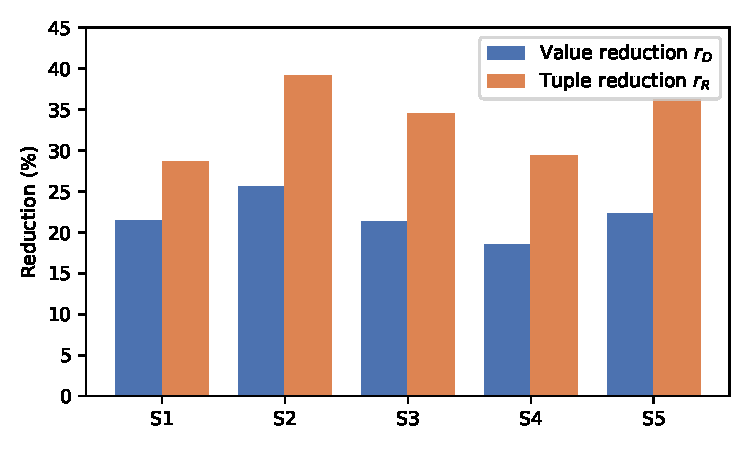
\includegraphics[
  width=\columnwidth
]{artifacts/figures/fig1_reduction.pdf}
\caption{
Domain and relation-table reductions obtained by generalized arc
consistency.
}
\label{fig:domain-reduction}
\end{figure}

\subsection{Static-suite feasibility and latency}

Table~\ref{tab:main-results} reports integer decision outcomes. The
conflict-unaware utility decoder directly produced a valid joint
assignment on only 2 of 250 instances. \method repaired the remaining
248 candidates and achieved 100\% verified feasibility.

The two unarbitrated sanity-check policies are reported separately in
Table~\ref{tab:sanity}, because they carry no verifier and therefore
cannot produce a pipeline outcome in the sense of
Table~\ref{tab:main-results}. What they measure is the rate at which
raw proposals happen to satisfy the registered model: zero of 250 in
both cases. Under the common forwarding gate, such outputs are not
admitted, since the gate admits only verifier-accepted candidates.

\begin{table}[t]
\centering
\caption{Sanity-check policies without arbitration. The reported
quantity is the number of raw policy outputs that satisfy the
registered hard model, not a pipeline outcome.}
\label{tab:sanity}
\setlength{\tabcolsep}{4pt}
\small
\begin{tabular}{lr}
\toprule
Raw policy & Registered-model feasible outputs\\
\midrule
Uncoordinated & 0/250\\
Static priority & 0/250\\
\bottomrule
\end{tabular}
\end{table}

Complete \cpsat and \gac followed by full \cpsat also achieved 100\%
verified feasibility. Their median latencies were 2.8 and 2.6~ms,
respectively, compared with 1.8~ms for \method.

\begin{table*}[t]
\centering
\caption{
Coordination-pipeline outcomes on the static suite, covering instance
update through repair and excluding independent verification,
certificate serialization, and E2 transport. Deadline compliance is
post-hoc. Sanity-check policies are reported separately in
Table~\ref{tab:sanity}.
}
\label{tab:main-results}
\setlength{\tabcolsep}{3pt}
\footnotesize

\begin{tabular}{lrrrrrrrrrr}
\toprule
Method &
$N$ &
Direct &
Local &
Full &
Fallback &
Blocked &
Feasible &
$\leq100$ ms &
Median &
P95\\
&
&
&
repair &
scope &
&
&
(\%) &
(\%) &
(ms) &
(ms)\\
\midrule


\gac + utility decode
& 250 & 2 & 0 & 0 & 0 & 248 & 0.8 & -- & -- & --\\

\cpsat
& 250 & 0 & 0 & 250 & 0 & 0 & 100.0 & 100.0 & 2.8 & 4.8\\

\gac + \cpsat
& 250 & 2 & 0 & 248 & 0 & 0 & 100.0 & 100.0 & 2.6 & 4.7\\

\textbf{\method}
& 250 & 2 & 248 & 0 & 0 & 0 &
\textbf{100.0} &
\textbf{100.0} &
\textbf{1.8} &
\textbf{3.8}\\

\midrule

Continuous only
& 250 & 189 & 0 & 0 & 0 & 61 & 75.6 & 23.6 & 180.4 & 365.7\\

\gac + continuous decode
& 250 & 186 & 0 & 0 & 0 & 64 & 74.4 & 44.4 & 80.6 & 251.3\\

Continuous + repair (explanation)
& 250 & 186 & 57 & 0 & 0 & 7 & 97.2 & 57.4 & 79.9 & 253.3\\

Continuous + repair (radius)
& 250 & 186 & 57 & 0 & 0 & 7 & 97.2 & 57.0 & 82.6 & 251.9\\

Continuous + repair (assumption)
& 250 & 186 & 58 & 0 & 0 & 6 & 97.6 & 57.8 & 81.3 & 254.4\\

\bottomrule
\end{tabular}
\normalsize
\end{table*}

The paired median difference between \method and complete \cpsat was
$-0.85$~ms, with a bootstrap 95\% interval
$[-0.93,-0.72]$~ms. The paired Wilcoxon result was
$p\approx 7\cdot 10^{-34}$ and the matched-pairs rank-biserial correlation was $-0.89$.
This difference is statistically significant under the specified paired test, although operationally modest in magnitude.

\begin{table*}[t]
\centering
\caption{
Final certification status of completed lexicographic repair
sequences. A decision or epoch is LEX-OPTIMAL when every
lexicographic level of its repair returned \texttt{OPTIMAL};
FEASIBLE-NOT-CERTIFIED denotes a verifier-accepted incumbent
returned before full lexicographic certification. An episode is
counted as LEX-OPTIMAL only if every repaired epoch in that episode
achieved complete lexicographic certification. Counts are completed
repair episodes, not internal solver calls; each sequence comprises
one or more core-feasibility calls followed by up to three
objective-level optimizations.
}
\label{tab:epoch-status}
\setlength{\tabcolsep}{4pt}
\small
\begin{tabular}{llrrr}
\toprule
Campaign & \shortstack[l]{Inferential\\unit} & \shortstack[l]{Completed repair\\sequences} & \shortstack[l]{Fully lex-\\optimal} & \shortstack[l]{Feasible-not-\\certified} \\
\midrule
Static & decision & 248 & 248 & 0 \\
Dynamic & epoch & 14{,}755 & 14{,}755 & 0 \\
Sequential F5 subset & episode & 40 & 40 & 0 \\
\bottomrule
\end{tabular}
\end{table*}

\begin{table*}[t]
\centering
\caption{
Paired static-instance comparisons. Latency effect sizes are
matched-pairs rank-biserial correlations. HL denotes the
Hodges--Lehmann paired difference in milliseconds. When $b+c=0$ no
discordant pairs exist; the McNemar comparison is reported as
$p=1$ by convention and carries no evidence of superiority in either
direction.
}
\label{tab:stats-paired}
\setlength{\tabcolsep}{3pt}
\small

\begin{tabular}{lrrrrrrrrr}
\toprule
Comparison &
$N$ &
Feasibility A/B &
$b$ & $c$ &
$p_{\mathrm{McN}}$ &
Median A/B &
HL &
$p_{\mathrm{Wilc}}$ &
$r_{\mathrm{rb}}$\\
\midrule

\method vs \cpsat
& 250 & 100/100 & 0 & 0 & 1.000 & 1.76/2.76 &
$-0.85$ & $<10^{-33}$ & $-0.89$\\

\method vs \gac+\cpsat
& 250 & 100/100 & 0 & 0 & -- & 1.76/2.63 &
$-0.75$ & $<10^{-30}$ & $-0.85$\\

Continuous+repair vs \method
& 250 & 97.2/100 & 0 & 7 & 0.031 & 79.9/1.75 &
$+94$ & $<10^{-40}$ & $+1.0$\\

Continuous+repair vs \cpsat
& 250 & 97.2/100 & 0 & 7 & 0.031 & 79.9/2.76 &
$+93$ & $<10^{-40}$ & $+1.0$\\

\bottomrule
\end{tabular}
\normalsize
\end{table*}

The objective-inspired baselines also achieved 100\% verified
feasibility and retained approximately 64\% of preferred actions.
Their latency results were obtained in the secondary environment and
are not directly compared with results from the primary host.

The continuous-relaxation stage was counterproductive on this suite.
It increased median latency to approximately 80~ms, reduced post-hoc
deadline compliance to approximately 57\%, and left six or seven
instances blocked, depending on the core rule. Its feasibility deficit relative to the discrete pipeline was statistically significant (exact McNemar $p=0.016$ unadjusted, $p_{\mathrm{Holm}}=0.031$). It was therefore
excluded from the proposed operational pipeline.

For the continuous-relaxation evaluations, the upstream end-to-end coordination feasibility sample size is strictly $N=250$. However, the downstream KPM-analysis sample is $N=249$ because one verifier-accepted decision failed during the post-verification KPM simulation stage due to a simulator numerical error. A post-verification simulator error does not constitute a failure of the upstream coordination pipeline. The failed simulation concerns a single S5 instance that was verifier-accepted under both \method and the continuous variants; the \cpsat KPM simulation on the same generated instance completed, so its marginal sample remains $n=250$, whereas the \method sample excludes that instance ($n=249$) and the explanation-guided continuous sample excludes it as well ($n=242$ of its 243 verifier-accepted decisions). Missing simulator values were omitted pairwise in computations using decisions as the resampling unit, and all KPM intervals are marginal decision-level bootstrap intervals rather than paired-sample intervals.

\subsection{Repair-core ablation}
\label{sec:repair-ablation}

Table~\ref{tab:repair-results} compares repair-core strategies on all 248 repair candidates produced by the conflict-unaware utility decoder on the static suite. Fixed violated-scope and radius-zero repair succeeded on 227 of 248 cases (91.5\%), whereas the expanding variants succeeded on all 248. The exact paired McNemar comparison between explanation-guided and radius-zero repair contained 21 discordant pairs, all favouring explanation-guided repair ($b=0$, $c=21$), giving $p_{\mathrm{raw}}=9.5\cdot 10^{-7}$ and $p_{\mathrm{Holm}}=2.9\cdot 10^{-6}$ within family F2. The success-rate advantage of core expansion over fixed-scope repair is therefore statistically significant on this suite. This advantage is attributable to expansion itself rather than to explanation guidance specifically: the frontier, assumption-core, and full-scope strategies also resolved all 248 candidates. The specific benefit of explanation guidance is that it recovered the 21 missed candidates with markedly smaller final cores than full-scope solving.

\begin{table*}[t]
\centering
\caption{
Repair-core ablation. ``Used'' gives the number of expansions driven
by explanations (e), assumption cores (a), and the frontier rule (f).
}
\label{tab:repair-results}
\setlength{\tabcolsep}{5pt}
\small

\begin{tabular}{lrrrcr@{\hspace{7pt}}rrr}
\toprule
&
\multicolumn{5}{c}{Operational candidates (248)}
&
\multicolumn{3}{c}{Stress suite (50)}
\\
\cmidrule(r){2-6}
\cmidrule(l){7-9}

Strategy &
Success &
Final core &
Used &
Released &
Median &
Success &
Final core &
Median\\
&
(\%) &
&
(e/a/f) &
&
(ms) &
(\%) &
&
(ms)\\
\midrule

Violated
& 91.5 & 10 & 0/0/0 & 0.00 & 0.97
& 100 & 8 & 0.54\\

Radius 0
& 91.5 & 10 & 0/0/0 & 0.00 & 1.01
& 100 & 8 & 0.51\\

Radius 1
& 99.2 & 14.5 & 0/0/0 & 0.00 & 1.57
& 100 & 16 & 0.65\\

Radius 2
& 100.0 & 16 & 0/0/0 & 0.00 & 1.71
& 100 & 22 & 0.90\\

Frontier
& 100.0 & 11 & 0/0/21 & 0.48 & 1.23
& 100 & 8 & 0.64\\

Explanation
& 100.0 & 11 & 16/0/8 & 0.30 & 1.19
& 100 & 8 & 0.64\\

Assumption
& 100.0 & 10.5 & 0/21/0 & 0.15 & 2.44
& 100 & 8 & 2.50\\

Full scope
& 100.0 & 20 & 0/0/0 & 0.00 & 1.78
& 100 & 24 & 1.37\\

\bottomrule
\end{tabular}
\normalsize
\end{table*}

Explanation-guided expansion used a median final core of 11 variables,
compared with 16 for radius two and 20 for full-scope solving.
Full-scope repair required a median 1.78~ms, compared with 1.19~ms for
explanation-guided repair. The latency advantage of explanation-guided repair over full-scope solving is statistically significant ($p=8.0\cdot 10^{-34}$, matched-pairs rank-biserial correlation $-0.89$; family F3 in Table~\ref{tab:families}). Its final cores are moderately but significantly larger than the fixed violated-scope and radius-zero cores (family F4: $p_{\mathrm{Holm}}=1.4\cdot 10^{-4}$), which is the price of the expansions that recovered the 21 cases lost by fixed-scope repair.

\begin{figure}[t]
\centering
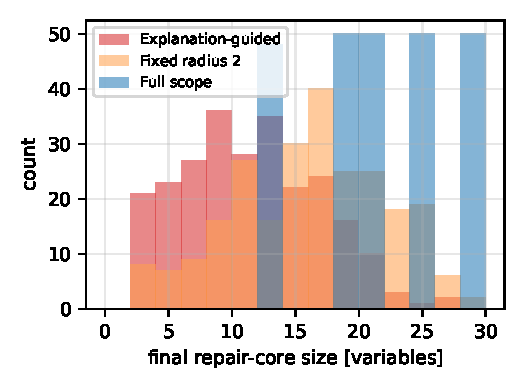
\includegraphics[
  width=\columnwidth
]{artifacts/figures/fig_core_sizes.pdf}
\caption{
Final repair-core sizes across the 248 operational-candidate repairs.
}
\label{fig:repair-core}
\end{figure}

These results concern candidates produced by the deliberately
conflict-unaware decoder. They demonstrate the effect of expansion
relative to fixed-boundary repair; they do not show that 248 repairs
would be required under a stronger operational decoder.

\subsection{Objective quality}
\label{sec:objective-quality}

The local repair boundary can exclude globally better solutions.
Across the static scenario suite, explanation-guided repair retained
53.8\% of preferred requests on average, whereas full objective
optimization retained 64.6\%. The mean difference was therefore 10.8
percentage points. The paired asymptotic Wilcoxon result was $p<10^{-35}$. Because 12.8\%
of paired differences were zero out of the $N=250$ static instances, the effective
non-zero sample was $N_{\mathrm{eff}}=218$; we used the asymptotic Wilcoxon signed-rank
test with \texttt{zero\_method='wilcox'}. The median paired gap was 11.2 percentage points (IQR: 6.8--14.5 percentage points) in favour of full optimization, with a matched-pairs rank-biserial correlation of $-0.92$. The gap did not exceed 40 percentage points.
Median latency was 1.25~ms for local repair and 2.21~ms for the full
objective optimizer. This 1.25~ms figure is not directly comparable
with the 1.19~ms reported in Section~\ref{sec:repair-ablation}: the
1.19~ms result concerns the repair-core strategy ablation, which
measures core feasibility only, whereas the 1.25~ms result belongs to
the separate objective-quality campaign and additionally includes the
operational lexicographic optimization stages.

Accordingly, the two capabilities should not be conflated. \method
provides verified feasible repair with an audit trace. A complete
objective solve provides global optimality when the solver returns the
required optimal status for the complete encoded objective.

\subsection{Incremental propagation}

Incremental propagation reproduced the fully recomputed filtered
domains on all 15{,}000 dynamic epochs.

\begin{table*}[t]
\centering
\caption{
Incremental propagation versus full recomputation. Times are mean
propagation times per epoch.
}
\label{tab:incremental-results}
\setlength{\tabcolsep}{4pt}
\small

\begin{tabular}{lrrrrrr}
\toprule
Transition &
Count &
Recomputed (ms) &
Incremental (ms) &
Gain (\%) &
Restored &
Agreement (\%)\\
\midrule

Base
& 150 & -- & -- & -- & -- & 100.0\\

Restrictive
& 750 & 0.102 & 0.014 & 86.3 & 0.00 & 100.0\\

Relaxing
& 750 & 0.100 & 0.050 & 50.2 & 0.38 & 100.0\\

Mixed
& 12{,}600 & 0.087 & 0.059 & 32.0 & 0.67 & 100.0\\

Utility-only
& 750 & 0.099 & 0.004 & 95.9 & 0.00 & 100.0\\

\bottomrule
\end{tabular}
\normalsize
\end{table*}

The largest relative reductions occurred for restrictive and
utility-only transitions. Relaxing and mixed transitions gained less
because the affected component was first restored. In absolute terms,
the savings were fractions of a millisecond. The larger sequential
benefit reported next is therefore mainly due to avoiding complete
model reconstruction and re-solving, rather than propagation alone.

\subsection{Conflict-aware decoders}
\label{sec:decoder-baselines}

The utility decoder is a weak candidate generator. Greedy checking,
min-conflicts, and forward checking were therefore evaluated on the
same 250 static instances.

\begin{table*}[t]
\centering
\caption{
Conflict-aware candidate generators. ``Direct'' is verifier-accepted
feasibility before repair. ``Repair needed'' is the number of
candidates subsequently passed to explanation-guided repair.
}
\label{tab:decoders}
\setlength{\tabcolsep}{3.5pt}
\small

\begin{tabular}{lrrrrrr}
\toprule
Decoder &
Direct &
Kept preference &
Median &
P95 &
Repair &
Median core\\
&
(\%) &
(\%) &
(ms) &
(ms) &
needed &
\\
\midrule

Utility decode
& 0.8 & 77.5 & 0.15 & 0.29 & 248 & 11\\

Greedy + checks
& 5.6 & 71.2 & 0.05 & 0.07 & 236 & 8\\

Min-conflicts
& 71.6 & 55.1 & 0.37 & 4.50 & 71 & 4\\

Forward checking
& 86.0 & 57.3 & 0.19 & 50.2 & 35 & 12\\

\bottomrule
\end{tabular}
\normalsize
\end{table*}

Min-conflicts and forward checking produced directly feasible
candidates on 71.6\% and 86.0\% of instances, respectively. Thus, the
248 repairs emphasized in the utility-decoder ablation should not be
read as the repair rate of the strongest evaluated candidate
generator.

Neither conflict-aware decoder eliminated repair. Forward checking
left 35 candidates unresolved within its 50~ms budget, and direct
feasibility fell from 100\% on S1 to 62\% on S5. Conflict-aware
decoders also retained fewer preferred values than the utility
decoder.

Explanation-guided repair completed the candidates from all four
decoders to 100\% verified feasibility in this suite. A practical
pipeline should therefore combine a conflict-aware candidate generator
with verified repair (see Section~\ref{sec:limitations} for the
decoder-dependence caveat).

\subsection{Cold-start and sequential operation}
\label{sec:sequential}
\label{sec:amortized-results}

Figure~\ref{fig:coldstart} reports the cold-start results over twenty
seeds per size. On isolated near-threshold instances, complete
\cpsat remained within the 100~ms post-hoc threshold up to
$n=1000$, with a median latency of 38~ms and a p95 of 43~ms.
The one-shot \method pipeline required a median of 68~ms and a p95 of
90~ms. Its observable Python \gac stage accounted for approximately
40\% of the measured cost.

Thus, the evaluated pipeline provides no cold-start latency advantage
over complete \cpsat for these isolated instances. A deployment that
faces unrelated coordination problems should use the complete solver
unless it requires another feature of the pipeline, such as its
verification or audit trace.

\begin{figure}[t]
\centering
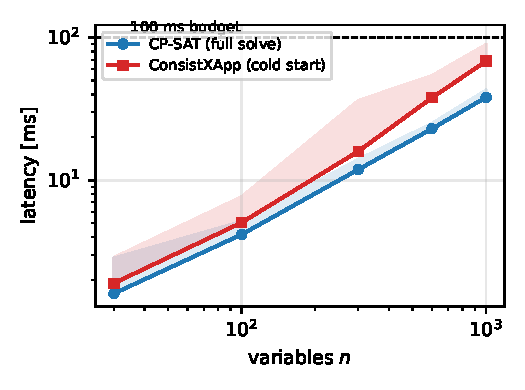
\includegraphics[
  width=\columnwidth
]{artifacts/figures/fig_coldstart.pdf}
\caption{
Cold-start latency on generated near-threshold instances. Lines show
medians and shaded regions extend to the pooled p95 over twenty seeds
per size. On these isolated instances, the one-shot \method pipeline
offers no latency advantage over complete \cpsat.
}
\label{fig:coldstart}
\end{figure}

The sequential experiment evaluates a different operating regime.
Consecutive epochs retain the same variables, domains, and utilities,
while a fraction of the registered relations changes. At each epoch,
the incremental strategy first re-verifies the previous verified
decision. If that decision violates the updated model, it is repaired.
The two comparison methods rebuild and solve the complete \cpsat
model, either without a hint or with the preceding solution supplied
as a hint.

The experiment is not a trivial re-verification workload. At
$n=1000$ and $\delta=2\%$, the previous decision remained feasible
without repair on only 1.7\% of epochs. At $n=100$, the corresponding
fraction was 69\%.

For $\delta=2\%$, verified incremental repair required a median of
0.05~ms per epoch at $n=100$ and 4.9~ms at $n=1000$. Rebuilding and
re-solving the complete model required medians from 2.8 to 25.6~ms.
The hinted rebuild-and-resolve baseline required medians from 2.9 to
27.4~ms.

All three methods reached 100\% verified feasibility on the evaluated
sequential epochs. Treating the episode as the inferential unit, the
per-episode median favoured incremental repair in all ten paired
episodes at each evaluated size and change rate. With ten non-zero
paired differences in the same direction, the two-sided exact
Wilcoxon signed-rank result attained its minimum possible value ($p=0.001953$) for ten pairs. Table~\ref{tab:sequential-stats} lists the resulting maximum Holm-adjusted $p$-values across all four evaluated configurations in comparison family F5. The exact tests handled zero differences by omitting them from the ranks, and no ties were present. The matched-pairs rank-biserial correlation was $-1.0$.

\begin{table*}[t]
\centering
\caption{Exact sequential Wilcoxon signed-rank results (Family F5). The Holm correction adjusts the raw exact $p=0.001953$ for four simultaneous comparisons.}
\label{tab:sequential-stats}
\setlength{\tabcolsep}{4pt}
\small
\begin{tabular}{llrrrc}
\toprule
Size &
Comparison &
Episodes &
Raw $p$ &
Holm $p$ &
$r_{\mathrm{rb}}$\\
\midrule
2\% / 100 & Incremental vs Re-solve & 10 & 0.001953 & 0.007812 & $-1.0$ \\
2\% / 300 & Incremental vs Re-solve & 10 & 0.001953 & 0.007812 & $-1.0$ \\
2\% / 600 & Incremental vs Re-solve & 10 & 0.001953 & 0.007812 & $-1.0$ \\
2\% / 1000 & Incremental vs Re-solve & 10 & 0.001953 & 0.007812 & $-1.0$ \\
\bottomrule
\end{tabular}
\normalsize
\end{table*}

At $n=1000$ and $\delta=2\%$, the Hodges--Lehmann estimate of the
per-epoch latency difference between incremental repair and
re-solving was $-20.3$~ms.

At $n=1000$, the unhinted re-solve spent a median of 6.9~ms
constructing the Python model and 18.4~ms in solver search. In this
implementation, both components scaled with complete model size, and
a solution hint removed neither model reconstruction nor complete
model processing (see Section~\ref{sec:limitations} for the scope of
this baseline).

\begin{figure}[t]
\centering
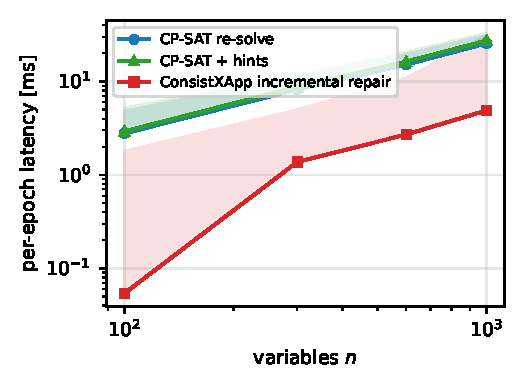
\includegraphics[
  width=\columnwidth
]{artifacts/figures/fig_amortized.pdf}
\caption{
Per-epoch latency when 2\% of the relations change between epochs.
Lines show pooled medians and shaded regions extend to the pooled p95.
The methods use identical generated episodes. The figure describes
the evaluated Python implementations and is not a hard real-time
guarantee.
}
\label{fig:amortized}
\end{figure}

\begin{table*}[t]
\centering
\caption{
Per-epoch latency over ten paired episodes of thirty epochs. Entries
are pooled median and p95 in milliseconds; the value after the
semicolon for incremental repair is the pooled p99. All strategies
reached 100\% verified feasibility. Because epochs within an episode
are dependent and only 300 epochs are available per configuration,
p95 and especially p99 are descriptive rather than precise tail
estimates. Drift rows re-plant 1\% of variables per epoch.
}
\label{tab:amortized}
\setlength{\tabcolsep}{6pt}
\small

\begin{tabular}{lrrr}
\toprule
Change / size &
\cpsat re-solve &
\cpsat + hints &
Incremental repair\\
\midrule

2\% / 100
& 2.8 (4.8)
& 2.9 (5.2)
& \textbf{0.05} (1.8; 4.4)\\

2\% / 300
& 8.2 (11.4)
& 8.7 (11.8)
& \textbf{1.4} (5.0; 13.2)\\

2\% / 600
& 15.2 (19.5)
& 16.3 (20.7)
& \textbf{2.7} (10.9; 22.7)\\

2\% / 1000
& 25.6 (31.2)
& 27.4 (32.8)
& \textbf{4.9} (30.6; 83.7)\\

10\% / 1000
& 18.3 (27.1)
& 20.2 (28.6)
& \textbf{4.5} (59.6; 137.8)\\

\midrule

Drift / 600
& 17.8 (20.9)
& 18.9 (22.0)
& \textbf{4.0} (25.8; 69.3)\\

Drift / 1000
& 28.1 (32.5)
& 29.8 (34.2)
& \textbf{9.8} (43.8; 81.3)\\

\bottomrule
\end{tabular}
\normalsize
\end{table*}

The pooled tail measurements reveal an important limitation. At
$n=1000$ and $\delta=2\%$, the p95 values of incremental repair and
unhinted re-solving were 30.6 and 31.2~ms, respectively. The pooled
p99 values were approximately 84 and 33~ms, and the largest observed
incremental-repair latency was 129~ms. At $\delta=10\%$, the pooled
incremental-repair p95 increased to approximately 60~ms.

These observations suggest that core growth can remove the median
advantage on difficult epochs; the small number of extreme
observations underlying the pooled p99 is discussed in
Section~\ref{sec:limitations}.

The drift variant reduces the risk that a fixed planted assignment
makes sequential repair artificially easy. Re-planting 1\% of the
variables invalidated the previous decision on every epoch. At
$n=1000$, incremental repair still had a lower median latency,
9.8~ms compared with 28.1~ms for unhinted re-solving. Its pooled p95
and p99 were nevertheless 43.8 and 81.3~ms, preserving the same tail
qualification.

Separately from the operational lexicographic pipeline, a diagnostic
temporal-stability sweep evaluated the scalarized formulation
$U-\mu H$ of \eqref{eq:problem-objective} on the dynamic sequence.
Increasing the churn weight $\mu$ from zero to one reduced mean action
churn by 11\%, while measured throughput changed by less than 0.2\%
and registered-model feasibility was preserved. The sweep therefore
characterizes the scalarized diagnostic model, not the lexicographic
operational objective, whose ordering is invariant to positive
scaling of the primary level. This is a result of
the synthetic pseudo-physical model and should not be interpreted as
a physical-network performance guarantee.

\subsection{Network-level descriptive results}
\label{sec:kpi-results}

Table~\ref{tab:kpi} reports descriptive KPM estimates for
verifier-accepted decisions. These values were generated by the
pseudo-physical model. They are not measurements from an emulated or
deployed O-RAN system.

\begin{table*}[t]
\centering
\caption{
Descriptive KPMs of verifier-accepted decisions, presented as preliminary diagnostic evidence, reported as mean and
bootstrap 95\% interval. Energy is measured in $\mu$J/bit. The
continuous-repair sample contains 242 verified decisions. One S5
\method KPM evaluation failed numerically after verification; the
\cpsat KPM for that instance remained available. The raw
uncoordinated proposal had a counterfactual mean throughput of
11.7~Mbps, but no uncoordinated proposal was accepted for execution.
}
\label{tab:kpi}
\setlength{\tabcolsep}{4pt}
\small

\begin{tabular}{lrrr}
\toprule
Method &
Throughput (Mbps) &
Energy ($\mu$J/bit) &
Jain fairness\\
\midrule

\cpsat{} ($n=250$)
&
10.84 [10.56, 11.12]
&
50.8 [49.6, 52.1]
&
0.443 [0.433, 0.452]
\\

\method ($n=249$)
&
10.41 [10.15, 10.68]
&
52.2 [51.0, 53.5]
&
0.433 [0.424, 0.443]
\\

\shortstack[l]{Continuous relaxation +\\explanation-guided repair ($n=242$)}
&
10.93 [10.68, 11.18]
&
50.6 [49.3, 51.9]
&
0.451 [0.441, 0.461]
\\

\bottomrule
\end{tabular}
\normalsize
\end{table*}

The marginal bootstrap intervals overlap for some KPMs, but overlap
of separate confidence intervals is not a paired equivalence test and
does not establish absence of a material difference. No
non-inferiority or equivalence margin was defined before analysis.
Consequently, Table~\ref{tab:kpi} supports only a descriptive
comparison.

The principal experimentally supported distinction is registered-model
feasibility, not KPM superiority; the additional evidence needed for
KPM equivalence claims is stated in Section~\ref{sec:limitations}.

% ============================================================
\section{Limitations and Threats to Validity}
\label{sec:limitations}
% ============================================================

This section is the single authoritative statement of the validity
caveats of this study; earlier sections refer here rather than
restating them.

\subsection{Registered-model validity}

Every formal guarantee in this paper is conditional on the registered
model. A verified decision satisfies the registered domains,
relations, model version, and context. It is not thereby safe for a
physical RAN if the model omits a relevant dependency or uses an
invalid threshold.

This limitation is particularly important for implicit conflicts,
whose representation depends on the quality of a parameter--KPM
model, validated profile, digital twin, simulator, or conservative
operator rule. The independent verifier checks consistency with the
registered representation; it does not validate the representation
against physical reality.

Model-version binding is also required to prevent a
time-of-check/time-of-use inconsistency. A candidate verified against
one model version must not be forwarded after the registered model
has changed unless it is re-verified.

\subsection{Verifier evidence}

The verifier-validation gates provide substantial implementation
evidence but do not constitute a proof of universal correctness. The
oracle, production verifier, and declarative implementation are
independent at the parser and checking levels, but the generated test
distribution still limits the conclusions.

Input mutation tests the classification of modified inputs. It is not
code-mutation testing and does not measure how many implementation
faults the test suite would detect. Zero divergence over 680{,}450
checks therefore means zero observed disagreement on the tested
inputs, not zero probability of an undiscovered defect.

\subsection{Local consistency and repair completeness}

\gac is a local property. Non-empty filtered domains do not establish
global feasibility. Similarly, infeasibility of a proper-core repair
model may be caused by fixed boundary values and does not establish
infeasibility of the complete registered model.

Conditional completeness applies only after expansion to the complete
variable set, exact encoding of the registered finite-domain
relations, and a conclusive solver status before the time limit.
A solver status of \texttt{UNKNOWN} must not be interpreted as
infeasibility.

The operational audit certificates establish replayable feasibility
and expansion traces. They do not establish minimum repair-core size
or global objective optimality. Certificate serialization size and
replay latency were not separately measured.

\subsection{Objective encoding and solver status}

The operational repair stage uses a lexicographic preference order,
but feasibility and optimality must be distinguished. A
\texttt{FEASIBLE} \cpsat result establishes a feasible assignment,
whereas an \texttt{OPTIMAL} result is required to establish
optimality for the encoded objective.

The separate objective-gap experiment compares repair with a complete
objective optimizer. Any final archival artifact must record the
integer scaling, coefficient bounds, lexicographic encoding, solver
status, time limit, number of search workers, random seed, and
presolve settings used in that experiment. Without these details,
the reproducibility package is incomplete.

\subsection{Decoder dependence}

The utility decoder was deliberately conflict-unaware. It generated
248 repair cases out of 250 instances, whereas forward checking
reduced the number requiring repair to 35. Therefore, the headline
repair count measures the contribution of repair under that weak
decoder, not the repair frequency of the strongest candidate generator.

The conflict-aware decoder experiment shows that repair remains useful,
but the large-scale sequential campaign was not repeated with every
decoder. A production evaluation should combine a conflict-aware
candidate generator with verified repair and should report end-to-end
latency, repair frequency, objective quality, certificate size, and
tail behaviour for that complete pipeline.

\subsection{Generated-instance structure}

The scale experiments use planted-feasible positive-table instances
with fixed domain size, relation count, and tightness. These choices
make coordination failures distinguishable from model infeasibility,
but they may favour local repair.

The experiments do not systematically vary graph density, clustering,
relation arity, domain size, tightness, feasible-region fragmentation,
or the distance between consecutive feasible regions. They also do
not evaluate large-scale sequences in which domains, xApp activation,
utilities, and relations all change simultaneously.

The sequential conclusion must therefore be restricted to the
evaluated generated workloads. It does not establish the same scaling
behaviour for dense, high-arity, adversarial, or commercial
multi-vendor O-RAN models.

\subsection{Baseline scope and latency measurement}
\label{sec:baseline-scope}

This subsection is the authoritative treatment of baseline scope;
earlier mentions are deliberately brief and defer here.

The sequential baselines rebuild their Python \cpsat models at every
epoch. The hinted variant adds the previous solution as a hint but
does not preserve a persistent solver state. Consequently, the
experiment compares \method with rebuild-and-resolve \cpsat, with and
without hints. It does not rule out faster persistent, incremental, or
lower-level solver implementations. We do not claim that no persistent
approach exists: we claim only that the evaluated Python
rebuild-and-resolve implementations behave as reported. A solver-native
large-neighbourhood baseline centred on the previous decision, and a
persistent model supporting in-place relation mutation, are the two
most informative comparisons not carried out here.

Reported latencies follow the decomposition of
Equation~\eqref{eq:latency-decomp} and exclude independent
verification, certificate serialization, and E2 transport. They are
therefore computational coordination latencies rather than
closed-loop control delays.

The campaigns also ran in two documented execution environments.
Paired comparisons remain within an environment, but absolute
latencies across environments are not directly comparable. A
single-host replication with fixed CPU affinity, warm-up,
garbage-collection policy, and repeated timing runs would strengthen
the systems conclusions.

\subsection{Tail latency and real-time interpretation}

The median sequential advantage is supported at the episode level.
The p95, p99, and maximum results are descriptive pooled-epoch
statistics. In particular, the p99 estimate for a 300-epoch
configuration is determined by approximately three observations and
has no reported dependence-aware uncertainty interval.

The 100~ms threshold is post-hoc. A stage can exceed the threshold
before the overrun is detected. Hence, the current implementation
does not provide a hard real-time guarantee, even though all verified
decisions in several campaigns completed within 100~ms.

A production architecture requires a preemptive budget policy, for
example per-stage time reservations, a solver limit based on remaining
budget, an already verified fallback, or an escalation rule triggered
by repair-core growth. No concrete tail-bounding policy was evaluated
in this study.

\subsection{Simulation and O-RAN deployment validity}

The pseudo-physical model does not capture E2 transport delay,
Near-RT RIC scheduling, container interference, message loss,
hardware acceleration, or vendor-specific O-CU/O-DU/O-RU behaviour.
The reported latencies are computational pipeline measurements, not
complete closed-loop control delays.

No claim of physical-network safety, KPM equivalence, or deployment
readiness follows from the current experiments. Closed-loop
validation on an O-RAN emulator or experimental platform is required.

% ============================================================
\section{Conclusion}
\label{sec:conclusion}
% ============================================================

This paper formulated registered multi-xApp arbitration in the Near-RT RIC as a dynamic finite-domain constraint problem and presented \method, a pipeline whose core contribution is an independently validated forwarding verifier with replayable audit certificates, supported upstream by incremental generalized arc consistency and explanation-guided repair. The stated formal properties---soundness of the forwarding gate relative to the registered model, solution preservation under filtering, and conditional completeness of expanding repair cores---are standard, but they delimit precisely what the architecture does and does not guarantee.

The production verifier showed zero divergence over 680{,}450 checks against multiple independent implementations and oracles, providing substantial implementation-level agreement on the tested generated inputs. On 250 generated static instances in a single-worker deterministic environment (num\_search\_workers = 1), \method reached a median computational latency of 1.8~ms. Thus, \method outperformed the evaluated Python rebuild-and-resolve \cpsat implementations on the generated sequential workloads. The operational pipeline repaired all 248 utility-decoder candidates. Across these repairs, explanation-guided expansion used markedly smaller cores than full-scope solving and succeeded on 21 candidates where fixed-scope repair failed. Stronger conflict-aware candidate generators substantially reduced the need for repair altogether.

The principal observed advantage was sequential and amortized. When 2\% of relations changed between generated epochs, incremental repair required median latencies of 0.05--4.9~ms for 100--1{,}000 variables, compared with 2.8--25.6~ms for rebuilding and re-solving. This median advantage was consistent across paired episodes, demonstrating the efficiency of exploiting temporal stability when successive control requests largely preserve the previous constraints and assignments. At 1{,}000 variables with 2\% relation changes, however, incremental-repair latency approached re-solve latency near the pooled p95 and exceeded it at the descriptive pooled p99.

However, several operational boundaries remain. Cold-start instances are better served by complete solving, local repair necessarily trades objective quality for speed (retaining fewer preferred requests than global optimization), and the observed median latency advantages do not constitute hard real-time tail guarantees. Future work will integrate conflict-aware decoding and verified repair as a unified pipeline, measure serialization overheads for audit certificates, evaluate denser constraint models, and perform closed-loop validation on O-RAN emulators and experimental testbeds.

% ============================================================
\section*{Statements and Declarations}
% ============================================================

\subsection*{Funding}

No funding was received for conducting this study.

\subsection*{Competing interests}

The authors declare that they have no competing financial or
non-financial interests that are directly or indirectly related to
this work.

\subsection*{Author contributions}

\textbf{Lillia Ouali:} Conceptualization, Validation, Supervision. \textbf{Madani Bezoui:} Conceptualization, Methodology, Formal analysis, Software, Investigation, Validation, Visualization, Writing -- original draft, Writing -- review \& editing. \textbf{Kamal Amroun:} Validation, Writing -- review \& editing. \textbf{Ahcene Bounceur:} Validation, Supervision. All authors reviewed and approved the manuscript.

\subsection*{Data and code availability}

The code, generated instances, raw logs, explanation traces,
verifier-validation reports, reproducibility manifests, seed
hierarchy, command lines, and scripts reproducing the tables, figures,
and statistical tests are available in the public repository:
\url{https://github.com/MadBezoui/OpenRanXAPP}.

The review artifact records the exact solver configuration for every
campaign, including time limits, worker counts, random seeds,
presolve settings, objective scaling, and solver statuses, in its
reproducibility manifests.

\subsection*{Ethics approval}

Not applicable.

\subsection*{Consent to participate}

Not applicable.

\subsection*{Consent for publication}

Not applicable.

\subsection*{Use of generative artificial intelligence}

Generative language models were used to assist with manuscript
organization, language editing, and review of analysis scripts. The
authors reviewed and corrected the resulting material and assume full
responsibility for the scientific content, formal statements,
references, experimental protocol, numerical results, and submitted
version.

\bibliography{references}

\end{document}
